% General document style ------------------------------------------------------------------
\documentclass[jou]{apa6}
%\documentclass[man]{apa6}
\usepackage[T1]{fontenc}
\usepackage[utf8]{inputenc}
%\usepackage{enumerate}

% Quotes
\usepackage{csquotes}

% Colors
\usepackage[usenames,dvipsnames]{color}

% Let us have multiline comments
\usepackage{verbatim}

% Footnotes in section headings
\usepackage[stable]{footmisc}

% Formatting bibliography
\usepackage[
    style=authoryear-comp,
    uniquename=false,
    url=false,
    maxbibnames=20,
    giveninits=true,
    isbn=false, backend=biber]{biblatex}
\addbibresource{gistr.bib}

% Mathematics, Code and tables
\usepackage{amsmath}
%\usepackage{bm}
%\usepackage{amsfonts}
\usepackage[group-separator={,}]{siunitx}
\usepackage{xfrac}
%\usepackage{mathtools}
\usepackage{alltt}
\usepackage{algorithm}
\usepackage{algpseudocode}
\usepackage{multirow}

\usepackage{listings}
\lstset{
    basicstyle=\ttfamily
}

% Have graphics
\graphicspath{{images/manual/}{images/computed/}}
\usepackage{subfig}
\usepackage{caption}
\captionsetup[subfloat]{margin=0.5em}

% Be smart with ref names
\usepackage{cleveref}

% Help in placing the floats
\usepackage{placeins}

% Have numbered quotes
\setlength{\leftmargini}{3em}
\newsavebox\nquotebox
\newenvironment{nquote}
  {\begin{equation}
   \begin{lrbox}{\nquotebox}
   \begin{minipage}{\dimexpr\columnwidth-2\leftmargini}
   \setlength{\leftmargini}{0pt}%
   \begin{quote}}
  {\end{quote}
   \end{minipage}
   \end{lrbox}\makebox[0pt]{\usebox{\nquotebox}}
   \end{equation}}

% To make comments, corrections, notes
\newcommand{\tb}[1]{\textcolor{blue}{#1}}
\newcommand{\rk}[1]{\tb{{\footnotesize {\bf[\emph{#1}]}}}}
\newcommand{\marginnote}[1]{\marginpar{{\parbox{1.\linewidth}{\hrulefill\\\tb{\scriptsize \sf #1}}}}}
\newcommand{\cam}[1]{\tb{\small{[{\bf C:} }#1{]}}}
\newcommand{\seb}[1]{\tb{\small{[{\bf S:} #1{]}}}}

% If citations or references are missing, make it visible
\newcommand{\CN}{\textsuperscript{\tb{[Citation needed]}}}
\newcommand{\CNs}{\textsuperscript{\tb{[Multiple citations needed]}}}

% Fix subsubsection to look as requested for submission
%\renewcommand{\typesectitle}[1]{#1\hfill\\ \vskip0.2\baselineskip \hskip-1em}

% Add figure placement indications in apamode "man"
\newcommand{\indicatemanfigure}[1]{
\ifapamode{%man
  \begin{center}
    -------------------------- Insert Figure \ref{#1} about here --------------------------
  \end{center}
}{%jou
}{%doc
}}


% Start with the real content -------------------------------------------------------------

\title{Transformations in large-scale text transmission chains}
\shorttitle{Gistr}
\date{}
\twoauthors{Sébastien Lerique}{Camille Roth}
\twoaffiliations{Seb's affiliations}{Cam's affiliations}
\abstract{
\rk{todo}
}
\authornote{\emph{Keywords:} \rk{todo}\\\emph{Corresponding author:} \rk{todo}}

\setcounter{secnumdepth}{3}

\begin{document}
\maketitle

% Use the following to tinker with section numbering, sometimes necessary for submission
% % Force section numbering
% \setcounter{secnumdepth}{3}
% % Remove section numbering for references
% \setcounter{secnumdepth}{0}

% The actual contents
\section{Introduction}\label{sec:gistr-intro}

The previous chapter demonstrated that it is possible to observe
cognitive biases in the way quotations are copied from blog to blog. By
grounding those biases in known effects in the recall of word lists, we
also showed that the enquiry of cultural evolution for linguistic
content can be related to lower-level cognitive mechanisms that help
understand the way content is transformed in ecological situations.
However in the online corpus we considered only extremely simple
transformations, namely individual word replacements, so as to be able
to infer missing links between quotations and thus make the analysis
possible. While we observed a reliable bias in the way words are
replaced, consistent with known psycholinguistic biases, our view of the
overall transformations is extremely narrow: not only is it restricted
to word replacements, it is limited to the replacements that were the
only change in an utterance (other than sentence cropping). The analysis
also remained at the low-level of lexical properties such as word
frequency and age of acquisition, neither of which give much insight
into the semantic changes that utterances can undergo. Finally,
constraints of the data did not let us identify chains of
transformations, and we could not observe the evolution of quotations
beyond the individual transformation step.

We now wish to remedy most of these points by studying the evolution of
short utterances in a controlled experimental setting. A controlled
setting means having a less ecological situation, but also allows for
the collection of all the available data for analysis. Once again, our
approach is exploratory, and we aim to reach a more complete
understanding of the transformation process that is at work in the
propagation of online quotations, but also more widely in the evolution
of written utterances as they are transmitted using other mediums. Our
reasoning is that by better understanding the transformations undergone
by such utterances, we will gain insight into the way actual linguistic
representations may change because of interpretation and memory
mechanisms.

More precisely, our goal is to construct a descriptive model of the
process that can bring insight into why utterances change the way they
do, and how such observations can be connected to current knowledge in
linguistics, on one side, and to the broader cultural evolution
frameworks, on the other. Indeed, current knowledge of the
transformation of utterances is quite partial: laboratory transmission
chains show that a number of high-level biases appear in the
transmission of purposefully constructed complex stories, but do not
explain in detail how such trends come about. On the other hand, the
psycholinguistics literature on sentence recall shows that there are
important semantic and syntactic effects in the way sentences are
reformulated, but they do so on extremely simple types of content that
make it difficult to generalise results. There seems to be a missing
link between the high-level effects observed in
transmission chains of complex stories and the lower-level processes known to act in the recall of simple sentences. A descriptive
model of transformations would go a long way in creating this link, and thus hope to explain more easily the overall evolution of utterances in terms of lower-level cognitive mechanisms.

One of the ideal setups to tackle this question would be a standard transmission
chain where we observe the accumulated transformations made by
participants on a set of utterances that we choose. 
%However, given our exploratory approach and the fact that we do not know in advance what the model will look like, it is important that we can run several such experiments in short cycles so as to adjust the task parameters and the sampling of utterances. It is also important that the collected data be of similar size to the number of substitutions we extracted in the previous chapter, so that we will be able to compare and validate any overlapping results. 
We chose to run a set of transmission chain experiments on an online platform developed for the purpose: as we shall see, after an initial development phase this approach lets us collect large amounts of data in short periods of time, while maintaining a level of control similar to that of laboratory experiments.

We begin by discussing the works relevant to this endeavour, and in
particular the bind in which current transmission chain experiments on
linguistic content find themselves. We then present the procedure
followed to develop the online experimental platform, and the measures
implemented to achieve a high level of quality in the data. Next, we
expose our analysis of the data sets collected, present the descriptive
model of transformations we construct from them, and highlight the main
behaviours the model lets us observe. Finally, we discuss the relevance
of these results in the broader context of the study of cultural
evolution.

\section{Related work}\label{sec:gistr-related}

Inspired by the selectionist models of culture developed by
\textcite{boyd_culture_1985} and
\textcite{cavalli-sforza_cultural_1981}, a sizeable part of the
empirical work on cultural change has focused on identifying content and
context biases in the way cultural items are transmitted. This line of
work relies heavily on the transmission chain paradigm initially
introduced by \textcite{bartlett_remembering:_1995}. For linguistic
content in particular, studies using that paradigm now provide a
catalogue of contrasts in the way utterances or short stories are
transmitted. These effects range from the stereotypical personification
of objects \autocite{bangerter_transformation_2000}, the favouring of
negative story aspects \autocite{bebbington_sky_2017} or the increased
hierarchical encoding of events \autocite{mesoudi_hierarchical_2004}, to
biases in favour of social \autocite{mesoudi_bias_2006} or
counter-intuitive aspects of stories
\autocites{norenzayan_memory_2006}{barrett_spreading_2001}. Other
effects such as the role of emotions in the selection of items to
reproduce \autocites{heath_emotional_2001}{eriksson_corpses_2014}, or
conformity and prestige biases \autocite{acerbi_did_2017} have been
studied by focusing on the individual transmission step on which the
evolution of content hinges.

Often, such effects are identified by selecting two or more minimally
different types of content and contrasting the way they evolve in
transmission chains (for instance measuring the rate at which they are
degraded). When a type of content is significantly better transmitted
than other types, it signals that a bias is acting on that contrast
dimension. The technique is useful in the context of selectionist models
of culture, as it identifies examples of biases which could create
selection pressures for specific cultural types and thus drive cultural
evolution. It is also relevant to the Cultural Attraction framework,
which focuses on the aspects of culture for which reconstructive
processes are more important than selection. For instance, the approach
introduced recently by \textcite{claidiere_how_2014} proposes to
use evolutionary causal matrices to model such attraction-based
processes in cultural evolution, and could gain insight from the trends
observed in transmission chains. In the terminology of
\textcite{morin_how_2016}, selectionist models focus on how culture
survives in spite of wear-and-tear, and cultural attraction focuses on
how culture survives in spite of possible flops, where a given item
fails to elicit sufficient interest to be recreated at all. In theory,
both selection and attraction can be observed in transmission chains. However, in
its current implementation focused on contrasting outcomes between
several (usually two) conditions, the technique gives little insight
into the underlying mechanisms at work, and how exactly such processes
can be described and explained in terms of cognitive %and situated
processing.

Indeed, understanding the mechanisms behind transformations in chains, or even only quantitatively describing the details of said transformations, remains very much a challenge.  This is especially true in the linguistic domain where the complexity of language hinders most attempts to comprehend sentence evolution.  Two typical strategies may be found in the literature. The first one trivially consists in doing the analysis by hand.  Here, we may further distinguish approaches relying on in vitro content, stemming from ad hoc experiments where participants have been asked to reformulate content under certain conditions, from approaches using in vivo content, stemming from generally large text datasets.
For instance, the study of risk perception propagation developed by \textcite{moussaid_amplification_2015} used a free-form interaction setting where subjects were filmed while freely discussing a topic. The recorded conversations were later hand-coded for the presence of certain information items introduced at the beginning of the chains. On the in vivo side, \textcite{lauf_analyzing_2013} carried out the linguistic analysis of transformations of quotes in a corpus of news stories by exhaustively hand-coding differences between sentences.

The second strategy consists in using automated methods.  In the in vivo case, this generally requires to focus on a tightly constrained type of transformation, and possibly rely on some empirical proxies, as there is no control on the conditions of production of the observed sentences. %It also relies on pre-labelled data sets, often from online platforms, on which machine learning techniques can extract features that correlate to the transmission of pieces of content. 
\textcite{danescu-niculescu-mizil_you_2012}, for instance, study the memorability of movie quotes by exploiting user ratings provided on the Internet Movie Database website. While their study does not focus on the transformation of content per se, it illustrates the types of memory-related features that %pre-labelled data sets can help extract in order 
may help explain transformations. Our analysis of single word substitutions in quotations observed in a large blog post dataset \autocite{lerique-2018-semantic-drift} belongs to this category as well.

In an in vitro setting, the only type of observed linguistic content evolution relies on single words –-- either in the case of intrusions in the recall of word lists \autocite[see][for a review]{zaromb_temporal_2006} and that of word replacements in short sentences \autocites{potter_regeneration_1990}{lombardi_regeneration_1992}.
%These studies can be seen as employing that strategy: 
These are much simpler processes than transformations of complete sentences, and are thus more amenable to statistical analysis. Note that a similar strategy is found in non-linguistic studies, such as iterated learning on sequences of colour items for which standard regularity metrics exist \autocite{cornish_systems_2013}, or transmission chains of constrained visual patterns such as those used by \textcite{claidiere_cultural_2014}. Both cases feature discrete and combinatorial pieces of content, for which it is possible to use natural notions of distance, equality, or regularity in transformation. 



%In an in vitro setting, the only type of observed linguistic content evolution relies on single words –-- either in the case of the study of intrusions in the recall of word lists \autocite[see][for a review]{zaromb_temporal_2006}, and that of word replacements in short sentences \autocites{potter_regeneration_1990}{lombardi_regeneration_1992} 
%%These studies can be seen as employing that strategy: 
%--- word intrusions in lists and individual replacements in sentences 
%both processes are much simpler than transformations of complete sentences, and are thus more amenable to statistical analysis. To the best of our knowledge, no experimental study has so far described sophisticated transformations at the sentence level in an automated manner.
%%In other words, automated analysis of in vitro content tightly constrains the linguistic features, for instance sentences of a very specific type, or for which only pre-defined changes can happen. %In that case the transformations can be directly modelled to identify regularities. 



%%Indeed, understanding the mechanisms behind transformations in chains,
%%or even only quantitatively describing the details of said
%%transformations, remains very much a challenge. This is especially true
%%in the linguistic domain, where the complexity of language hinders most
%%attempts to understand what is going on in a transformation. Up to now
%%three main strategies have been developed to delve into to detail of
%%transformations. The first is to use tightly constrained linguistic
%%content, for instance sentences of a very specific type, or for which
%%only pre-defined changes can happen. In that case the transformations
%%can be directly modelled to identify regularities. The study of
%%intrusions in the recall of word lists \autocite[see][for a
%%review]{zaromb_temporal_2006}, and that of word replacements in short
%%sentences
%%\autocites{potter_regeneration_1990}{lombardi_regeneration_1992}, can be
%%seen as employing that strategy: word intrusions in lists and individual
%%replacements in sentences are much simpler than transformations of
%%complete sentences, and are thus more amenable to statistical analysis.
%%Our analysis of single word substitutions in quotations observe in a large blog post dataset \autocite{lerique-2018-semantic-drift} can be categorised here too. A similar strategy is found in non-linguistic
%%studies, such as iterated learning on sequences of colour items for
%%which standard regularity metrics exist \autocite{cornish_systems_2013},
%%or transmission chains of constrained visual patterns such as those used
%%by \textcite{claidiere_cultural_2014}. Both cases feature discrete and
%%combinatorial pieces of content, for which it is possible to use natural
%%notions of distance, equality, or regularity in transformation. This
%%first strategy can be termed the \enquote{simple setting} strategy.
%%
%%At the other end of the spectrum we find the \enquote{do-it-by-hand}
%%strategy. This approach uses more ecological content but relies on
%%exhaustively hand-coding it, and is used in most of the transmission
%%chain studies mentioned above. The study of risk perception propagation
%%developed by \textcite{moussaid_amplification_2015}, for instance, used
%%a free-form interaction setting where subjects were taped while freely
%%discussing a topic. The recorded conversations were later hand-coded for
%%the presence of certain information items introduced at the beginning of
%%the chains. The linguistic analysis of transformations of quotes in news
%%stories provided by \textcite{lauf_analyzing_2013} is also the product
%%of exhaustively hand-coding differences between sentences.
%%
%%Finally, the third strategy relies on pre-labelled data sets, often from
%%online platforms, on which machine learning techniques can extract
%%features that correlate to the transmission of pieces of content. This
%%is the \enquote{already coded} strategy.
%%\textcite{danescu-niculescu-mizil_you_2012}, for instance, study the
%%memorability of movie quotes by exploiting user ratings provided on the
%%Internet Movie Database website. While their study does not focus on the
%%transformation of content per se, it illustrates the types of
%%memory-related features that pre-labelled data sets can help extract in
%%order to explain transformations. Conversely, analysing the regularities
%%that arise in unlabelled digital traces often falls back into the first
%%strategy: without an outsourced coding of the data, analysing
%%unconstrained real-life interactions is so complex that one often has to
%%focus on a limited set of features in the available data, thus proposing
%%a \enquote{simple setting} analysis. As we saw in the previous chapter,
%%the analysis of partial digital traces can also fall back into the first
%%strategy, as having to infer missing information led to drastically
%%simplifying the transformations considered.
%%
%%Strategies two and three are additionally closely tied to data
%%collection methods. Free-form interaction and more generally ecological
%%content is costly to hand-code, and thus necessarily limited in size; it
%%is also best used in controlled settings where the choice of content can
%%be optimised. Conversely, using machine learning to extract features
%%that relate to content transmission requires large amounts of
%%pre-labelled data, which often means that an existing public data set
%%must be used. Such studies thus seldom control the conditions under
%%which the data is generated, which restricts the interactions they can
%%explore to those encoded in existing data sets: any behaviour or piece
%%of content that is not observable in public data sets is off limits.

%%Overall, studies targeted at understanding the details of
%%transformations of linguistic content seem forced to pick two of the
%%following three properties, and relinquish the third: realistic content,
%%computational analysis, and control over the generation of the data.
%%Picking \enquote{realistic content and computational analysis} leads to
%%the \enquote{already coded} strategy. Picking \enquote{realistic content
%%and control over data generation} requires hand-coding a substantial
%%part of the data collected, that is strategy two. Finally,
%%\enquote{computational analysis and data generation control} leads to
%%the \enquote{simple setting} strategy. This bind thus appears as a major
%%challenge to the better understanding of changes in linguistic content,
%%and more broadly to the study of language-related cultural evolution. In
%%particular, it hinders attempts to model the low-level processes which
%%could provide a more parsimonious account of the contrasts observed in
%%linguistic transmission chains, and allow for a deeper integration of
%%the study of cultural evolution with linguistics.

To the best of our knowledge, no experimental study has so far described sophisticated transformations at the sentence level in an automated manner. 
To overcome this obstacle we turn to two related fields of research. The
first, which we term the Web and Smartphone experimental approach, %is creating a middle ground between controlled laboratory experiments and the analysis of online corpora. This approach 
takes advantage of the ubiquity of internet browsers and mobile computing to develop
large-scale controlled experiments out of the laboratory.
\textcite{miller_smartphone_2012} %discusses the possibilities opened by developing experiments as smartphone applications in particular, and
notes that this method changes the logistics %and context-awareness 
of experiments: large amounts of subjects can be recruited online without
having to manage meeting schedules, %, and experiments can probe
%participants without interrupting their everyday life, both 
advantages
that have been exploited in the study of mind-wandering and happiness
\autocites{killingsworth_wandering_2010}{mackerron_happiness_2013}{bastian_language_2017},
%A closely related method is the development of experiments as web
%applications, which similarly changes the set of experimental
%constraints. 
%In linguistics, the possibility for large-scale data
%collection has been successfully used in 
 vocabulary size
\autocites{keuleers_word_2015}{brysbaert_how_2016}, %; creating studies
%that involve many subjects at the same time is also made much simpler by
%the online logistics, an advantage that has been used for instance in
%the study of
or group conversations \autocite[][which also involves many subjects simultaneously]{niculae_conversational_2016}.
%More generally, these approaches relax the opposition between
%small-scale controlled experiments in the laboratory on one side, and
%analyses of large-scale but passively collected online data on the other
%side. 
Once the initial development cost is covered, they make it
possible to collect relatively large data sets in short cycles, and
combine simplified logistics with a level of control similar to that of
laboratory experiments.

The second field we rely on creates an opening for the detailed
modelling of utterance transformations: biological sequence alignment,
the sub-field of bioinformatics which seeks to uncover commonalities in
sequences of DNA, RNA, or amino acids in proteins from different
species, has developed over the last 50 years a range of general
algorithms to relate sequences of items. One such algorithm in
particular, introduced by \textcite{needleman_general_1970}, extends the
principles of the Levenshtein distance and is particularly well suited
to the analysis of linguistic transformations when combined with
standard natural language processing methods. Inspired by
\textcite{lauf_analyzing_2013} who use similar tools to prepare their
data for manual analysis, we use and extend the Needleman-Wunsch
algorithm to reliably extract regularities in the way utterances are
transformed through transmission chains.

\section{Methods}\label{sec:gistr-methods}

\subsection{Experiment design
principles}\label{experiment-design-principles}

\subsubsection{Advantages and challenges of transmission
chains}\label{advantages-and-challenges-of-transmission-chains}

An obvious way to address the questions raised in the previous chapter
is to use transmission chains in the laboratory to study the evolution
of online quotations in a controlled setting: each subject reads,
retains, and rewrites sentences that are then passed on to the next
subject in a chain of reformulations. Such a setup can reproduce an
idealised version of the read-remember-rewrite process which, we
hypothesised, participates in the evolution of quotations in blogspace
and media outlets. It also provides the information that our previous
data set lacked in order to analyse the complete transformations of
quotations, as well as the long-term effect of those changes: the links
between parent and child sentences are naturally encoded in the data,
such that the transformations undergone by each sentence can be studied
in full detail. There is no need to restrict ourselves to simpler
changes as was necessary for the inference procedure used with digital
traces from blogspace. By creating an artificial setting, the experiment
design also lets us control the reading and writing conditions as well
as the context in which sentences appear, which further removes one of
the inevitable uncertainties of the previous protocol (albeit at the
cost of less ecological conditions).

However, the laboratory transmission chain paradigm is not a good fit
for our exploratory approach: we aim to collect data that will allow us
to study both the complete set of transformations undergone by short
utterances such as online quotations, and the interactions and
cumulative effect of such changes; yet we do not know in advance the
types of changes that subjects will make, or the extent to which such
changes vary according to the type of linguistic content. Transmission
chain studies typically start with an a priori hypothesis focused on a
well-identified type of content, which is then empirically tested by
contrasting the evolutionary outcome of two classes of sentences.
Instead, our goal here is to provide first steps to characterise the
process by which such evolution of linguistic content arises, and
observe how it accumulates in the long term. The setup must thus allow
us to collect enough data to extract regularities in successive
transformations operated by different subjects on different sentences,
and provide a resolving power similar to that of substitutions in online
quotations so that we can compare results with the previous chapter.
Since our main target is the set of detailed transformations and their
interactions, a phenomenon of higher dimensionality than the contrast of
accumulated outcomes, it is also crucial to fine-tune the difficulty of
the read-write task and the complexity of the source sentences, in order
to trigger a set of transformations varied enough that it could approach
some of the changes encountered in real life situations. Our progress
therefore involves a non-trivial trial-and-error component: indeed, a
task made too easy or too difficult, and more so a set of source
sentences that are too complex or too straightforward, will lead to
either mass deletions or perfect conservation (or the former followed by
the latter), none of which can help characterise the more intricate
changes that linguistic content undergoes in the ecological setting we
aim to simulate.

%%\subsubsection{Web and smartphone experiments}\label{web-and-smartphone-experiments}
%%
%%Complementary to laboratory studies and to approaches using online
%%digital traces, a new empirical approach based on Web browsers and
%%mobile computing is striking a different balance in the trade-offs of
%%experimental work; it seems very promising in addressing the problems
%%outlined above. Indeed, browsers (both on desktop and mobile) and
%%smartphones have evolved into powerful, ubiquitous application
%%environments for which one can develop any kind of experiment involving
%%text, graphics, and human interactions. At the cost of increased
%%engineering requirements and a different approach to subject
%%recruitment, Web and smartphone experiments give the designer full
%%control over what data is collected and the way interactions are framed
%%(similar to laboratory experiments), and make it possible to quickly
%%collect data sets at scales comparable to what filtered and cleaned
%%digital traces provide.
%%
%%This approach makes a number of unusual trade-offs, the benefits of
%%which can be summarised as follows:
%%
%%\begin{itemize}
%%\item
%%  \emph{Control}: similar to laboratory experiments, and unlike digital
%%  trace analysis, it is possible to use complex designs where all the
%%  interactions of the subjects are framed and observed by the
%%  experimenter. This includes for instance the presentation of the
%%  experiment (e.g.~as a game or a self-improvement aid, aside from being
%%  a scientific study) and, more importantly, the ways in which the
%%  system mediates the interactions between the subjects.
%%\item
%%  \emph{Scale}: if and when needed, the technical platform can scale the
%%  number of subjects to the tens of thousands at low marginal cost.
%%  Interactions between subjects can also scale to involve synchronous or
%%  asynchronous contact between hundreds of people, without having to
%%  manage per-subject scheduling.
%%\item
%%  \emph{Speed of data collection}: once the initial development is
%%  completed (see costs below), the data collection cycle is short. One
%%  day can be enough to collect \num{1000}--\num{10000} usable data
%%  points, a size comparable to the final substitutions set extracted and
%%  analysed in the previous chapter. This is especially relevant for
%%  exploratory work which is made much easier with shorter
%%  trial-and-error cycles.
%%\item
%%  \emph{Flexible recruitment}: while also a challenge (see costs below),
%%  subject recruitment is more flexible than in the laboratory: services
%%  like Prolific Academic\footnote{\url{https://www.prolific.ac/}.} let
%%  the experimenter recruit at reasonable costs in pools of tens of
%%  thousands of subjects with fine-grained demographic filters. Wider
%%  audiences can be achieved by offering non-financial rewards, framing
%%  the experiment as a self-improvement application, or turning it into a
%%  game.
%%\end{itemize}
%%
%%The corresponding costs are the following:
%%
%%\begin{itemize}
%%\item
%%  \emph{Technical challenge}: developing Web and smartphone experiments
%%  involves a substantial amount of engineering, and makes use of
%%  technologies that most researchers, even technical, are not familiar
%%  with. While a couple of all-in-one kits exist,\footnote{See e.g.
%%    \url{http://funf.org/} and \url{http://www.epicollect.net/}.}
%%  creating an experiment that meets one's research questions requires
%%  learning average skills in most of the technologies at play: a native
%%  or cross-platform smartphone development environment, Web application
%%  development, backend server programming, and some server
%%  administration skills. Most importantly, the paradigms and problems
%%  encountered are new to researchers: control flow is asynchronous due
%%  to network communication and the user interface, and technicalities
%%  such as user management or email validation can grow into difficult
%%  engineering challenges.
%%\item
%%  \emph{Spam-control}: subjects are not constrained or encouraged by the
%%  face-to-face interaction of a laboratory experiment, neither are they
%%  (in most experiments) in the course of an interaction with friends
%%  that provides natural incentives for what they write, as can be the
%%  case with digital traces. Participants must have an incentive to
%%  perform the experiment's tasks well. If the spam introduced by one
%%  subject can be isolated in the design of the experiment, one
%%  possibility is to filter it after data collection and make payment
%%  depend on its prevalence. But if the spam introduced by one subject
%%  naturally propagates to data seen by other subjects in the experiment,
%%  as is the case for transmission chains, effective anti-spam pressures
%%  and motivations need to be factored into the design.
%%\item
%%  \emph{Recruitment cost}: while recruiting up to a few hundred subjects
%%  is cheaper than the equivalent for a laboratory experiment (not
%%  counting the development cost),\footnote{Global competition on online
%%    platforms like Prolific Academic drives subject payments down.} and
%%  is easy to manage for fast prototyping and pilot tests, recruitment
%%  cost rises linearly with the number of subjects and the time they
%%  spend on the experiment, unless a different strategy is used. Turning
%%  an experiment into a playful application or an application useful to
%%  the subjects (effectively making them users) involves yet another set
%%  of skills, can prove challenging, and must be factored into the
%%  development cost.
%%\end{itemize}

\subsubsection{General setup for Web-based transmission
chains}\label{general-setup-for-web-based-transmission-chains}

The balance achieved by Web-based experiments is well adapted to the
requirements we outlined above. Since no existing system would fit our
needs, we chose to develop a tailored Web-based platform that could run
transmission chains as Web experiments. Once ready, the platform would
allow us to gather sufficient amounts of quality data in short cycles.
We further decided to implement the simplest possible version of the
transmission chain paradigm that is still viable, and leave the
exploration of more complex setups for future research: the task we used
asks subjects to read and memorise a short utterance, wait a few
seconds, then rewrite what they have read as accurately as possible. We
ran three main experiments using this evolving platform, and many
smaller pilots in between to test lessons learned in the larger runs and
adjust task parameters and source complexity. The overall quality of the
data we gathered thus gradually increased. In what follows we present
the general setup of the experiments, the data quality evaluation along
with the changes implemented to improve it, and finally the adjustment
of task complexity. Let us start with the architecture common to all
experiments.

A transmission chain is defined by a type of content transmitted, a
transmission task, and a layout defining which subject production is
used as the source input for the next subject. In our implementation,
subjects are presented with an utterance to memorise with no surrounding
context; no distraction task is used between the reading and writing
phases, and the material incentive for the task is purely monetary
(although as we describe below we fine-tuned the interface to strongly
encourage subjects to be conscientious). The experiment is available to
subjects as a website, and passing it involves going through a welcome and sign-up screen, answering a preliminary questionnaire, and training for the main task, where subjects are asked to repeatedly
  memorise and rewrite short utterances as accurately as possible.
  As the instructions illustrated in \cref{fig:gistr-instructions}
  indicate, an utterance is presented to the subject and after a short
  pause they are asked to rewrite it as remembered. The process loops
  until the subject has completed all the utterances assigned to them
  (calibrated so that completing the experiment lasts at most one hour).
  The real trials started after 3 to 5 training trials, depending on the
  overall experiment length.

This simple setup lets us quickly gather data sets of several thousand
utterance transformations, ensuring our results will be comparable to
those from the set of \num{6177} substitutions extracted in the previous
chapter. Two parameters are then left to vary: the reading time for the
source utterances, computed as the number of words in an utterance
multiplied by a reading factor that is to be adjusted, and the set of
initial source utterances.

Each utterance from the initial set is used to create several parallel
chains in order to allow for comparisons across chains with the same
initial utterance. The final data thus consists of a set of
reformulation trees, where each tree branch is a transmission chain
started from the tree root, and continuing until it reaches a target
depth defined for the experiment. We therefore use the terms
  \enquote{chain} and \enquote{branch} interchangeably in what follows.
The number of branches in a tree is also adjusted for each run of the
experiment. Except for those who drop out before finishing the
experiment, all subjects are exposed exactly once to each tree in random
order, such that all the reformulations in a given tree are made by
distinct subjects, and nearly all subjects (excluding dropouts) are
present in each tree. Satisfying this constraint means that we must
always have at least as many subjects as there are reformulations in a
tree. As noted, a few subjects from Prolific Academic will usually not
complete the whole set of utterances assigned to them; we thus recruit
additional subjects to fill the trees that were left incomplete. This
leads the other, already complete trees to receive more reformulations
than needed, making some of their branches run a little deeper than the
target depth. All branches are cropped to the target depth for analysis.
\Cref{fig:gistr-trees}
shows a representation of the shape of the final trees.\footnote{Note that when exposed to a tree, subjects are always randomly
assigned to the tip of one of the branches that have not yet reached the
target depth: subjects are thus randomly distributed across branches,
but their depth-ordering loosely corresponds to the time of arrival on
the tree. In particular, if a subject starts the experiment after most
other subjects have completed it, they will be mostly exposed to
utterances deep in the branches. Due to the chained nature of the data,
there is no economical way of countering this ordering bias.}

%%\begin{figure}[!ht]
%%  \centering
%%  \subfloat[Welcome screen]{
%%    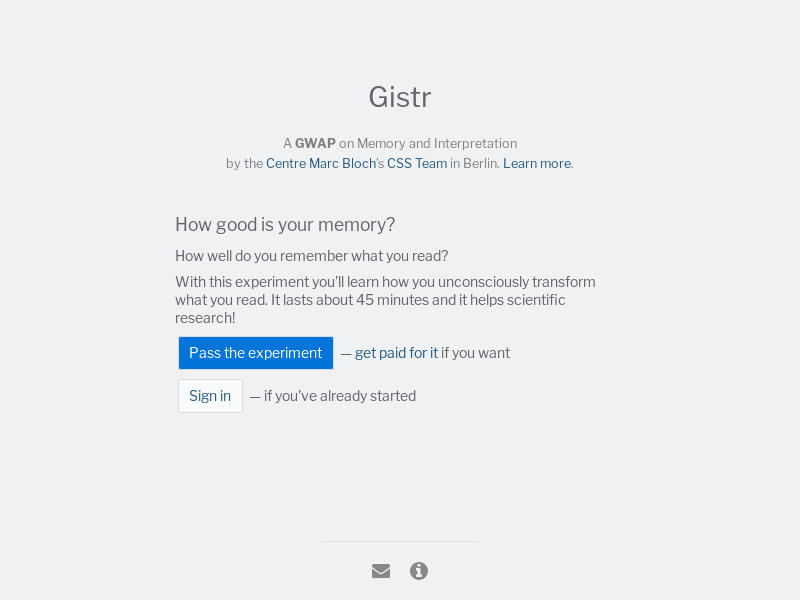
\includegraphics[width=.48\linewidth]{images/manual/gistr-welcome.png}
%%    \label{fig:gistr-welcome}
%%  }
%%  ~
%%  \subfloat[Signup form]{
%%    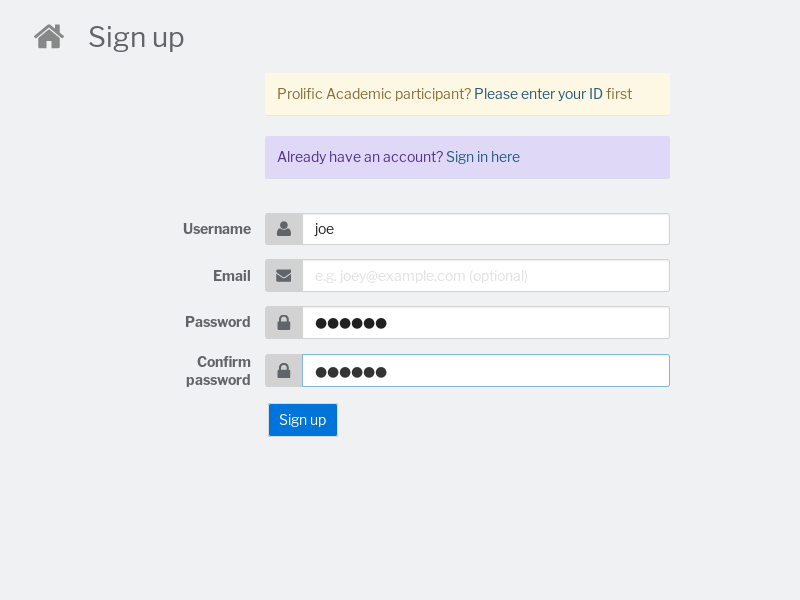
\includegraphics[width=.48\linewidth]{images/manual/gistr-signup.png}
%%    \label{fig:gistr-signup}
%%  }
%%  \caption[Initial steps for a subject entering the experiment]{
%%  \textbf{Initial steps for a subject entering the experiment.}
%%  }
%%  \label{fig:gistr-start}
%%\end{figure}
%%
%%\begin{figure}[!ht]
%%  \centering
%%  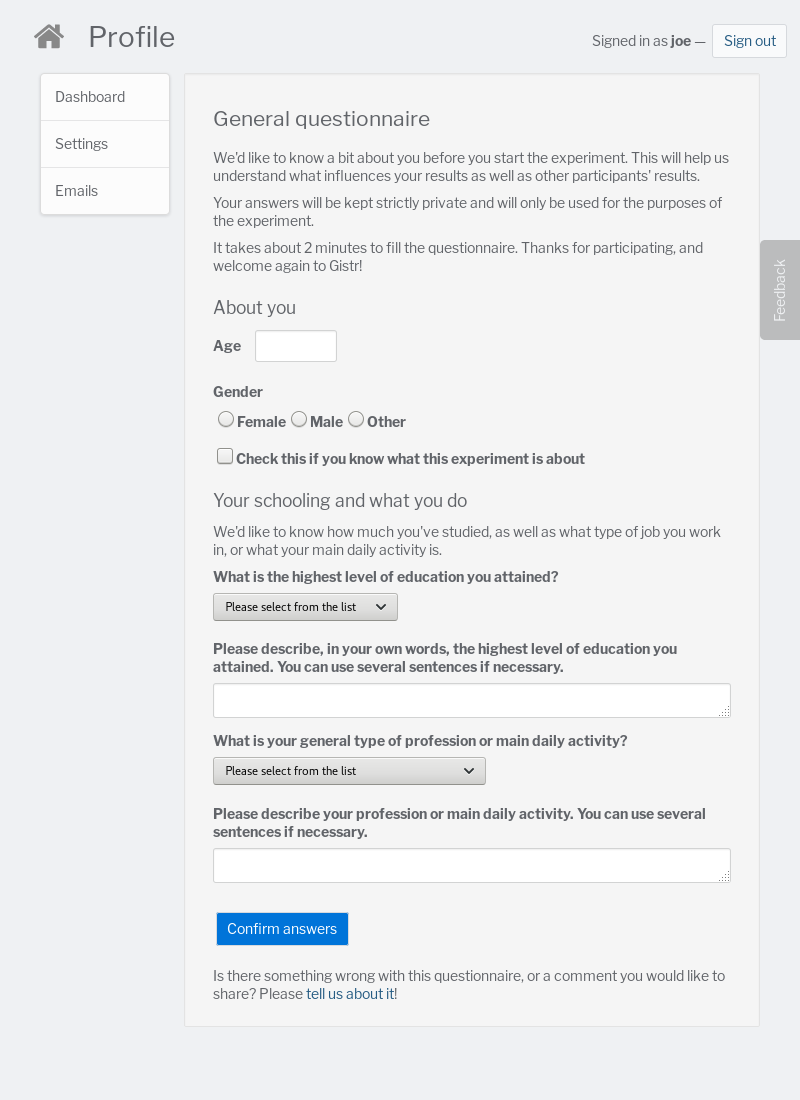
\includegraphics[width=.9\linewidth]{images/manual/gistr-questionnaire.png}
%%  \caption[Initial questionnaire]{
%%  \textbf{Initial questionnaire.}
%%  Subjects can additionally submit feedback on the questionnaire or any other aspect of the experiment on most screens of the website.
%%  }
%%  \label{fig:gistr-questionnaire}
%%\end{figure}

\begin{figure}[!ht]
  \centering
  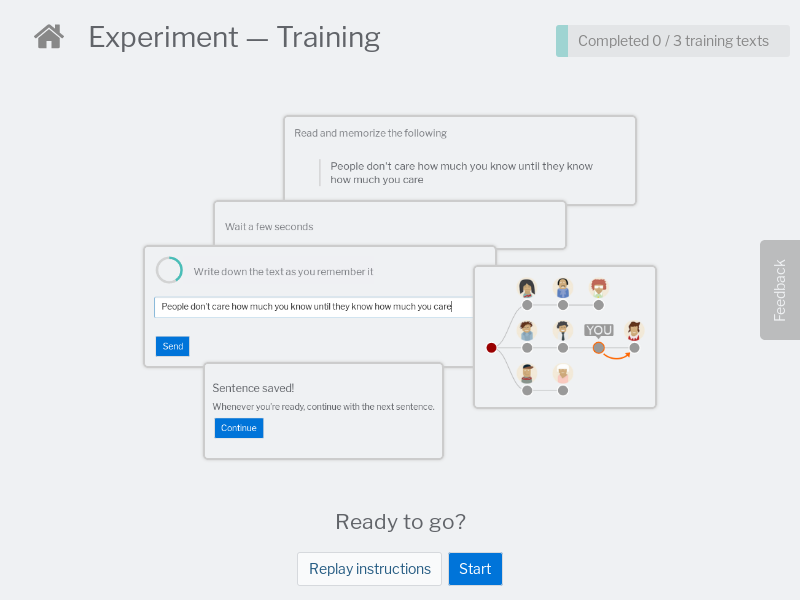
\includegraphics[width=.85\linewidth]{images/manual/gistr-instructions-training.png}
  \caption[Instructions for the main task]{
  \textbf{Instructions for the main task.}
  }
  \label{fig:gistr-instructions}
\end{figure}

\begin{figure}[!ht]
  \centering
  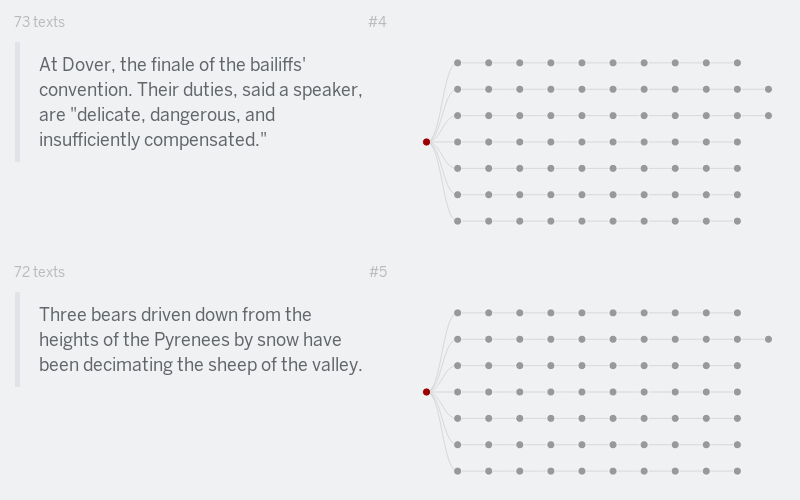
\includegraphics[width=.85\linewidth]{images/manual/gistr-trees.png}
  \caption[Example reformulation trees]{
  \textbf{Example reformulation trees.}
  Two example reformulation trees generated by the setup, targeted at 7 branches of depth 10:
  the text on the left is the initial utterance for all branches of a tree, represented by a red dot in the right-hand graph; each grey dot in the graph represents an utterance produced by a subject on the basis of the preceding dot.
  Subjects create at most one reformulation in each tree, and most create exactly one per tree.
  %The fact that some subjects drop out before completing all their trees leads us to recruit new subjects to fill in the missing reformulations, which is why some branches are uneven.
  }
  \label{fig:gistr-trees}
\end{figure}

Technically, the platform is a complete Web application based on current
technologies, with accompanying backend server to collect and distribute
utterances.
The experiment is available at \url{https://gistr.io} and subject
recruitment was done using Prolific Academic, a service analogous to
Amazon Mechanical Turk and geared towards academic research.

Using the Prolific Academic service allowed us to select among a pool of
over \num{26000} subjects, for which we used the following criteria: (i) first language English speaker, (ii) at least 18 years old, (iii) current country of residence and place of most time spent before
  turning 18 must both be in the UK, (iv) normal or corrected-to-normal vision, (v) no diagnosed literary difficulties, (vi) completed secondary school and (vii) not having participated in any of the preceding experiments.
Only the first two constraints were enforced for the first experiment,
and the full set was used for all subsequent runs. The full filter
provided over \num{2300} eligible subjects, from which the service
automatically sampled the request number of subjects we requested.

Experiment 1 was the first non-trivial launch of the platform, with an
initial 48 subjects, 54 root utterances, and trees targeted for 6
branches of depth 8. Subjects took an average 64 minutes to complete the
experiment, and were rewarded with £6.5. We gathered a total of 2695 utterance reformulations, slightly above the planned \(54 \times 6 \times 8 = 2592\) reformulations due to a minor technical issue. 
%%A software bug that appeared
%and had to be fixed halfway through the experiment led the Prolific
%Academic service to recruit more subjects than was originally asked for,
%and the final number of participants was 53,\footnote{The bug appeared
%  only once a large proportion of trees had reached their target depth,
%  and then affected all the subjects nearing completion of the
%  experiment. The time taken to respond to complaints and realise that
%  the experiment had to be paused led some subjects to exceed the
%  maximum allowed time on Prolific Academic, and the service then sent
%  the experiment out to new subjects. After fixing the bug, most
%  subjects who had started the experiment accepted to finish it, leading
%  the final subject count to be higher than originally requested.}
%gathering a total 2695 utterance reformulations (above the planned
%\(54 \times 6 \times 8 = 2592\) reformulations). 
Manual inspection
showed that large portions of the data were of poor quality, both
linguistically and because of technical inefficiencies leading to badly
shaped trees; the sections below provide further details on these
questions. Pilots following Experiment 1 were therefore aimed at
improving data quality and solving tree shaping issues. Experiment 2 was
launched with 49 subjects, 50 root utterances, and trees targeted for 7
branches of depth 7, gathering a total 2450 utterance transformations.
Subjects took an average 43 minutes to complete the experiment, and were
rewarded with £6. Quality issues in this data set were solved, but the
choice of source utterances proved too easy to trigger varied
transformations. After pilots exploring different fits of task
parameters with source complexity, Experiment 3 took advantage of a more
complex set of source utterances. It was launched with two batches of 70
subjects each receiving 25 root utterances, and trees targeted for 7
branches of depth 10, gathering a total 3546 utterance transformations.
Subjects took an average 37 minutes to complete the 25 transformations,
and were rewarded with £4.25 on average.

%We now detail the evaluation of data quality and the measures that were
%taken to improve it. The section after that will focus on the fit of
%task parameters and source complexity, before moving on to the analysis
%and results.

\subsection{Data quality}\label{data-quality}

The choice of a Web-based setup sets the requirements of the interface
much higher than for a laboratory experiment. There is no opportunity
for a face-to-face walk-through of the experiment or for questions, and
subtle changes in the way the interface reacts to actions can lead
subjects to interpret a signal where none was intended, or conversely to
not notice an important message. 
%%The time of the subjects is not booked,
%%and not having to travel to the laboratory or to talk to someone renders
%%the interaction free of any commitment and generally more consumable:
%%subjects can leave whenever they want, without having to feel bad about
%%it (the only cost being the loss of their reward). The lack of human
%%interaction with the experimenter also removes a natural incentive for
%%subjects to take their time and perform according to what the
%%experimenter in front of them explained. Combined together, these
%%factors mean that if the interface is strenuous or ambiguous in any way,
%%subjects will often pick the interpretations that make the process
%%faster and either complete the experiment with minimal engagement or
%%drop out. Redacting detailed textual instructions often makes matters
%%worse. Instead, t
The interface must lead the subjects through the
necessary explanations while remaining enjoyable, and must be
unambiguous while still hinting towards the expected behaviour at the
right moment, either through subtle interface reactions or through
explicit contextual aids.
%\subsubsection{Manual spam-coding}\label{manual-spam-coding}
Failure to properly encourage and wherever possible enforce the
experiment's expectations led to data riddled with spurious
transformations. Manual inspection of the data collected through
Experiment 1, for which a substantial effort on instructions and for the
overall interface had already been made, showed that large portions of
the data were not usable as such. 

We therefore spam-coded utterances for all experiments by hand. An utterance
with any of the following properties was coded as spam:
(i) 
  An ellipsis (\enquote{\ldots{}}) or other special characters (e.g.
  \enquote{\textgreater{}}, \enquote{\textless{}}) are present;
(ii)
  The utterance is partly or completely addressed to the experimenter
  (e.g. \enquote{Sorry, I can't remember});
(iii)
  Over half the words are misspelled;
(iv)
  The utterance has no relationship to its parent utterance (i.e.~it is
  an entirely new utterance);
(v)
  The utterance does not stand as an autonomous sentence, either because
  it is truncated or because so many words are garbled it becomes
  nonsense.
\footnote{Note that the last two criteria are not sharp, and several borderline
cases had to be decided for the last one in particular. In Experiment 1
for instance, a subtle misunderstanding allowed by the interface led
subjects to submit some sentences truncated at exactly 10 words, without
regard to their meaning (see the details below); such utterances were
unambiguously incomplete, and were thus coded as spam. In subsequent
experiments however, utterances that could be made complete with the
addition or the deletion of a single, sometimes unimportant word, were
questioned by the same criterion. For instance the simple sentence
\enquote{Mr Jones was robbed during} can be completed by adding the word
\enquote{dinner} at the end, or by removing the word \enquote{during}.
Such sentences do not seem tied to a misunderstanding of the task, and
are arguably attributable to temporary distraction whose effects are
relevant to our analysis. The benefit of the doubt was given to such
utterances, and they were not coded as spam.}
Spam in transmission chains has the additional property of invalidating
all the subsequent utterances, leading to discard more utterances than the ones where subjects introduced spam for the first time. 
Coded this way, Experiment 1 showed an accumulated spam rate of 22.4\%.
Combined with an initial technical oversight, where participants could concurrently participate in the same reformulation on the same branch and which led a small portion of
utterances to be misplaced in the chains,
%%\footnote{Ensuring that no two
%%  subjects are creating reformulations for the same chain tip at the
%%  same time, while not blocking other subjects from moving on with the
%%  experiment, is a non-trivial technical hurdle. Not solving it leads
%%  the chains to have \enquote{forks}, that is, utterances with several
%%  children (possibly extending to sub-branches) instead of a single one.
%%  One of the children must then be chosen to form the main chain, and
%%  the others discarded. Solutions to the problem are difficult to test
%%  in practice, as they involve simulating dozens of subjects
%%  concurrently sending utterances to the platform. The approach adopted
%%  in Experiment 1 relied on client-side randomisation, but proved
%%  insufficient: 3.5\% of the utterances posted by subjects were forks
%%  deep in the chains. Experiments 2 and 3 relied on a mix of client-side
%%  randomisation and server-side locking to solve the problem.} 
a total of 25.9\% of the utterances generated by Experiment 1 were discarded.
The number of valid transformations garnered by this experiment thus
went from 2695 to 1980. Apart from reducing the size of the usable data,
spam also leads to uneven chains across trees, a heterogeneity that
complicates the analysis. Accepting this level of spam was therefore not
an option.

The main tool we used to reduce the level of spam is the user interface.
As explained above, minor changes in the way the interface reacts to the
subjects' actions combined with relevant context-dependent information
can have a comparatively large impact on spam.
The situation is similar to that of surveys, where much effort is put
into mitigating the risk of users engaging the minimum possible effort
to complete the survey \autocite{krosnick_threat_2000}. Successfully
tuning the user interface is therefore a crucial factor in the quality
of the data collected: what the interface might lead subjects to see as
acceptable can easily be spam for the experimenter, and both
perspectives must be aligned as much as possible. Interface design
problems appeared repeatedly throughout the development of the platform
and the pilots. The most important points can be summed up as follows: 
(i) 
  \emph{Preventing digital copy-paste} (an obvious workaround)
  %: an obvious workaround to the
  %task that most subjects will try in the first few trials.
(ii)
  \emph{Avoiding signals that may be interpreted as a success} (such as avoiding to disable the ``send'' button below a certain number of words, which led some participants to validate their input as they reached the threshold);
%  : a well-known behaviour in transmission
%  chains of linguistic content is the rapid reduction in size of the
%  content that is transmitted
%  \autocites{maxwell_remembering_1936}{bangerter_transformation_2000}{mesoudi_hierarchical_2004}.
%  In order to encourage subjects to rely on what they remember, and
%  prevent them from quickly reaching empty sentences, an early version
%  of the experiment would disable the \enquote{send} button if the
%  subject's input was shorter than 10 words (Experiments 2 and 3 later
%  relaxed this constraint to 5 words). However, some subjects
%  interpreted the button becoming active after 10 words as a signal that
%  their input was ready to be sent as is, even if it was only a partial
%  sentence. This ambiguity, corrected in later versions, is responsible
%  for a large part of the spam found in Experiment 1.
(iii)
  \emph{Improving input quality} (including emphasizing the importance of transmitting correct sentences to the next participants); 
%  : Experiment 1 and subsequent pilots
%  showed the need for strong incentives to write well-edited meaningful
%  text. Indeed when pressed for time, some subjects will tend to write
%  misspelled, poorly punctuated, or even meaningless utterances, which
%  invalidate all the sentences that follow in the branch. Countering
%  this tendency involved several changes to Experiments 2 and 3:
%  emphasis was added to the fact that what is produced by one subject is
%  later sent to other subjects, encouraging a more conscientious
%  behaviour; a bonus was associated with high-fidelity trials, and the
%  top 5 subjects with lowest transformation rates (as defined below in
%  the analysis) received increased payment; most importantly, input from
%  the subjects was also checked for repeated or inadequate punctuation,
%  and for correct spelling against a combined British and American
%  English dictionary. The interface asked subjects to correct any input
%  that failed those tests, and presented them with a short explanation
%  that emphasised the faulty behaviour and recalled the chain structure
%  of the experiment. Inspecting the platform logs showed that this last
%  measure led subjects to often correct their utterances, a fact that
%  was also confirmed by the increased average writing time.
(iv)
  \emph{Relaxing the time pressure} (and avoiding rushed behaviors, by enforcing a minimal reading time);
%%  : the interface of Experiment 1 made
%%  several mistakes that worsened the inherent pressure on subjects to
%%  complete the study as fast as possible (indeed, payment on Prolific
%%  Academic is per experiment, not per time spent -- which, conversely,
%%  would encourage subjects to be very slow). First, subjects could
%%  terminate the reading time of an utterance at will. While this
%%  provided a measure of the effective reading time used by subjects, it
%%  also opened the possibility of speeding through the trials. Indeed
%%  over a third of the transformations of Experiment 1 were done by using
%%  less than half the allotted reading time. This pressure was increased
%%  by the presence of a \enquote{remaining time} clock in the reading and
%%  waiting phases, similar to the green clock shown on
%%  \cref{fig:gistr-instructions} for the writing phase. By removing
%%  superfluous clocks, keeping the reading time fixed, and proposing a
%%  break after each utterance, Experiments 2 and 3 relaxed the time
%%  pressure on the subjects and improved the final data quality.
(v) 
  \emph{Feedback channel} (for subjects to comment on the
  questions they were asked); and
%%  , and encourage the use of debriefing
%%  sessions to deepen that understanding
%%  \autocite{de_leeuw_international_2008}. Such feedback channels have
%%  also become a norm in online services, and we therefore chose to give
%%  the possibility for subjects to comment on most screens of the
%%  experiment (excluding the read-write screens) through a side-ribbon
%%  which, when clicked, would overlay a comment box (see
%%  \cref{fig:gistr-feedback}). It seems, however, that a more interactive
%%  option would be more effective, as only a handful of subjects entered
%%  comments over the course of Experiments 2 and 3.
(vi)  \emph{Instructions} (fine-tuning the exact phrasing of instructions and making it more ergonomic).
%% of the   making the
%%  interface for instructions palatable using a now common pattern: for
%%  the instructions pictured in \cref{fig:gistr-instructions} for
%%  instance, different elements or images are successively foregrounded
%%  and highlighted, and a tooltip with short explanations appears next to
%%  the active element.\footnote{The pattern was popularised by software
%%    libraries such as Intro.js (\url{http://introjs.com/}).} Here too,
%%  Experiment 1 and subsequent pilots allowed users to skip these
%%  instructions, leading a portion of the subjects to effectively never
%%  read them. Experiments 2 and 3 made navigating the complete list of
%%  instructions mandatory in order to start the trials.
%%\end{itemize}

These changes reduced the spam rate drastically. On the same criteria as
Experiment 1, Experiment 2 showed an accumulated spam rate of .8\%,
which combined with misplaced utterances led to a total 1.4\% of
utterances discarded (leading to a final 2411 valid transformations).
Experiment 3 showed an accumulated spam rate of 1.0\%, and with
misplaced utterances had to discard a total 1.1\% of the data (leading
to a final 3506 valid transformations).

%\begin{figure}[!ht]
%  \centering
%  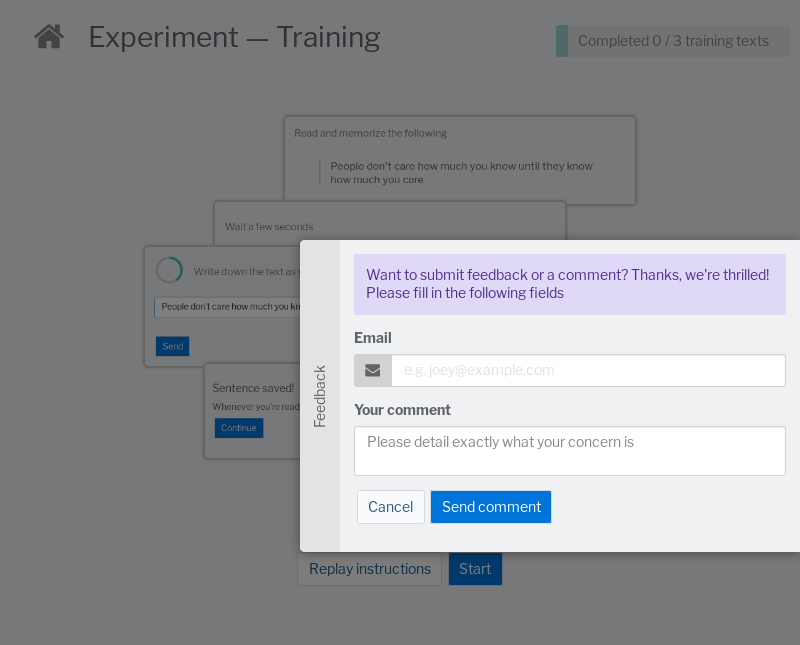
\includegraphics[width=.75\linewidth]{images/manual/gistr-feedback.png}
%  \caption[Overlay feedback box]{
%  \textbf{Overlay feedback box.}
%  Opened in the instructions screen from Fig.~\ref{fig:gistr-instructions}.
%  The box is available in most screens of Experiments 2 and 3.
%  }
%  \label{fig:gistr-feedback}
%\end{figure}
%
\subsection{Task difficulty and source complexity
fit}\label{task-difficulty-and-source-complexity-fit}

In the simple task we used, difficulty is controlled by the reading time
allotted to subjects and by the selection of source utterances. To unify reading times
 across utterances we made them proportional to the number of words \(|u|_w\) in a given utterance \(u\): 
reading time is defined as \(|u|_w \cdot r\), with \(r\) the
\emph{reading factor}. Average reading speeds for university students
are usually between 200 and 300 words per minute, that is between 3.33
and 5 words per second \autocite%[see][where fast readers average at 330~wpm and slow readers average at 207~wpm]
{rayner_eye_2010}. A reading factor of \(r = 1\) therefore gives fast readers the time to read
utterances more than 5 times, and slow readers about 3 to 4 times. A
reading factor of \(r = .3\) gives fast readers one or two readings, and
slow readers at least one. \(r = .2\) gives some readers one reading and
others less than one, and \(r = .1\) lets readers simply glance at the
utterances without being able to read them completely.

Pilots and manual exploration indicated that the difficulty of the task
is not linear with \(r\). Whatever the value of \(r\), longer utterances
(more than 25 words) are often more transformed, relative to their
length, than shorter utterances; longer utterances also give more space
for the subjects to reformulate, leading to more changes in style and
permutations in the words. Changing \(r\) has less effect on shorter
utterances than on longer utterances, and on utterances in oral versus
written style. For short utterances in an oral style, pilots indicated
that there is an abrupt transition between a low transformation regime
when subjects can read the sentence at least once, and an extremely
noisy regime when the subjects do not have the time to read the
utterances entirely at their normal speed. Conversely, the transition is
smoother for longer utterances or utterances with a more formal written
style. Choosing an adequate set of source utterances is therefore an
integral factor in adjusting the difficulty of the task.

Changing the source utterances also affects the sampling bias in ways
that are difficult to measure given the multidimensionality of text.
Contrasting minimally different utterances in different domains has
resulted in domain-specific outcomes on for instance stereotypes,
information hierarchy, and counter-intuitiveness
\autocites{kashima_maintaining_2000}{mesoudi_bias_2006}{barrett_spreading_2001}{mesoudi_multiple_2008},
and authors have suggested that these outcomes are related to
domain-specific biases in transformations (although to our knowledge
these effects have not yet been studied jointly). In spite of this, we
hypothesise that the low-level cognitive mechanisms underlying utterance
transformation, that is the mechanisms that give rise to such
accumulated outcomes, do not fundamentally change because of the type or
the style of an utterance. If using news quotes instead of movie quotes
or stories is likely to affect parameters of the observed
transformations, it is less likely to affect the structure of the
underlying cognitive mechanism, and therefore the general structure of
transformations. Making this hypothesis lets us use utterance selection
as an exploratory tool: by altering both the sampling of the
transformations and the task difficulty, the exploration of different
styles and types can help (1) improve data quality and (2) make the
general structure more visible, thus easier to measure and characterise.
%%\footnote{If this exploration yields insights about the structure of
%%transformations and their effects in the long term, and if such insights
%%are consistent with the previous chapter, then it will make sense to ask
%%to what extent the uncovered structure is applicable to or varies with
%%other types of utterances. Throughout pilots and experiments, our goal
%%was therefore to find a set of utterances which would trigger varied
%%transformations whose structure we could analyse, while at the same time
%%helping the subjects to produce quality data by not creating too much
%%pressure with reading time.}

The set of sources used in Experiment 1 covered a broad spectrum of
utterance types sampled from the following categories:

\begin{itemize}
\item
  Quotes found in blog posts from the MemeTracker data set \autocite{leskovec_meme-tracking_2009} and used in a recent article on sentence reformulation \autocite{lerique-2018-semantic-drift},
\item
  Famous compelling quotes from Wikisource\footnote{\url{https://en.wikisource.org/}.}
  such as \enquote{Never doubt that a small group of thoughtful
  committed citizens can change the world, it is the only thing that
  ever has},
\item
  Quotes extracted from the movie \emph{12 Angry Men} such as
  \enquote{If you ask me I'd slap those tough kids down before they
  start any trouble, it saves a lot of time and money},
\item
  Excerpts from news stories on controversial subjects (such as
  \enquote{How will the cultural and religious aspects of so many
  migrants impact E.U. society?}) or risk-related subjects such as
  stories about the risks of Triclosan \autocite%[used by][ in their  study of the amplification of risk perception]
{moussaid_amplification_2015},
\item
  The tale \enquote{War of the Ghosts} used by
  \textcite{bartlett_remembering:_1995} in his original
  studies,\footnote{Available online at
    \url{http://penta.ufrgs.br/edu/telelab/2/war-of-t.htm}.} as well as
  excerpts from other tales,
\item
  A small number of hand-crafted sentences such as surprising statements
  (\hbox{e.g.} \enquote{Don't forget to leave the door open when you leave the
  office}) or stereotype-incongruent statements (\hbox{e.g.} \enquote{The young
  boy was suddenly hit by the little girl}).
\end{itemize}

Each of these categories, we thought, could encourage the triggering of
transformations. The spam level of Experiment 1, and especially the
amount of misspelled words, made the exploration of the detailed
transformations impossible and shifted the focus towards improving data
quality through the interface. Nonetheless, it became clear that using
such a heterogeneous set of utterances could surprise subjects, and was
not the best approach to elicit regularities in transformations.
Experiments 2 and 3 relied on a more thorough exploration of possible
source data sets. Pilots explored utterances extracted from previous
studies \autocites[ on personification and increased
stereotypes]{bangerter_transformation_2000}[ on the role of
disgust]{heath_emotional_2001}[ on incoherent
stories]{maxwell_remembering_1936}[ for the role of social
information]{mesoudi_bias_2006}.

Two larger and more homogeneous sets of utterances were reconstituted
and finally used in Experiments 2 and 3. First, a set of movie quotes
provided by \textcite{danescu-niculescu-mizil_you_2012}. This data set
contains about 2200 pairs of quotes extracted from 1000 movie scripts;
each pair is made of a quote that was marked as memorable by users of
the Internet Movie Database, coupled with the closest quote in the same
movie script that is spoken by the same character, has the same number
of words, but is not marked as memorable on the Internet Movie Database.
The 2200 pairs of quotes were filtered to keep only those which passed
the spelling and punctuation quality tests from the previous section,
and for which the number of words was strictly matched when excluding
punctuation (this left 505 pairs). Here is an example pair from this
data set (first the memorable quote, then the non-memorable
counterpart):

\begin{quote}
\enquote{The first and most important rule of gunrunning is never get
shot with your own merchandise.}
\end{quote}

\begin{quote}
\enquote{At least when they say they're going to have a war, they keep
their word.}
\end{quote}

Second, a set of short stories from \textcite{feneon_novels_2007} was
used. These stories are productions from Félix Fénéon originally
anonymously published in the French newspaper \emph{Le Matin} in 1906.
They describe facts from everyday life such as accidents, suicides, or
trials, in a terse and sometimes humorous style. The following example
illustrates the style of these stories:

\begin{quote}
\enquote{An unidentified maker of paste jewels from the third district
was fishing in a boat with his wife at Maldon. She fell. He dived. Both
gone.}
\end{quote}

A sample of 60 stories was extracted from the English version, for which
French names and places were replaced with names and places more
familiar to British subjects. Pilots explored these sets of utterances
with reading factors of .1, .2, .3, .75 and 1. Finally, tests were also
made using these utterances with content words replaced with
pseudo-words, in order to restrict effects to the grammatical dimension
only.\footnote{Pseudo-words were generated using the Wuggy library
  \autocite{keuleers_wuggy:_2010}.} The pseudo-word tests turned out not
to fit our exploration framework however, as the task became too
confusing and subjects often replaced unknown words with real words.

Experiment 2 used 25 of the 27 pairs of movie quotes that had exactly 15
or 16 words, providing a homogeneous set of 50 utterances in oral style,
with a reading factor of .75. Experiment 3 used 43 of the 60 short
stories by Fénéon (average number of words \num{21.2}) coupled with 4
utterances extracted from \textcite{mesoudi_bias_2006} (average number
of words \num{60.3}) and 3 utterances extracted from the story used by
\textcite{maxwell_remembering_1936} (average number of words
\num{40.7}), with a reading factor of 1.







%%%%%%%%%%%%%%%%%%%%%%%%%%%%%%%%%%%%%%%%%%%%%%%%%%%%%%%%%%%%%%%%%%%%%%%%%%%
%%%%%%%%%%%%%%%%%%%%%%%%%%%%%%%%%%%%%%%%%%%%%%%%%%%%%%%%%%%%%%%%%%%%%%%%%%%
%%%%%%%%%%%%%%%%%%%%%%%%%%%%%%%%%%%%%%%%%%%%%%%%%%%%%%%%%%%%%%%%%%%%%%%%%%%
%%%%%%%%%%%%%%%%%%%%%%%%%%%%%%%%%%%%%%%%%%%%%%%%%%%%%%%%%%%%%%%%%%%%%%%%%%%
%%%%%%%%%%%%%%%%%%%%%%%%%%%%%%%%%%%%%%%%%%%%%%%%%%%%%%%%%%%%%%%%%%%%%%%%%%%
%%%%%%%%%%%%%%%%%%%%%%%%%%%%%%%%%%%%%%%%%%%%%%%%%%%%%%%%%%%%%%%%%%%%%%%%%%%
%%%%%%%%%%%%%%%%%%%%%%%%%%%%%%%%%%%%%%%%%%%%%%%%%%%%%%%%%%%%%%%%%%%%%%%%%%%
%%%%%%%%%%%%%%%%%%%%%%%%%%%%%%%%%%%%%%%%%%%%%%%%%%%%%%%%%%%%%%%%%%%%%%%%%%%
%%%%%%%%%%%%%%%%%%%%%%%%%%%%%%%%%%%%%%%%%%%%%%%%%%%%%%%%%%%%%%%%%%%%%%%%%%%
%%%%%%%%%%%%%%%%%%%%%%%%%%%%%%%%%%%%%%%%%%%%%%%%%%%%%%%%%%%%%%%%%%%%%%%%%%%
%%%%%%%%%%%%%%%%%%%%%%%%%%%%%%%%%%%%%%%%%%%%%%%%%%%%%%%%%%%%%%%%%%%%%%%%%%%
%%%%%%%%%%%%%%%%%%%%%%%%%%%%%%%%%%%%%%%%%%%%%%%%%%%%%%%%%%%%%%%%%%%%%%%%%%%
%%%%%%%%%%%%%%%%%%%%%%%%%%%%%%%%%%%%%%%%%%%%%%%%%%%%%%%%%%%%%%%%%%%%%%%%%%%
%%%%%%%%%%%%%%%%%%%%%%%%%%%%%%%%%%%%%%%%%%%%%%%%%%%%%%%%%%%%%%%%%%%%%%%%%%%
%%%%%%%%%%%%%%%%%%%%%%%%%%%%%%%%%%%%%%%%%%%%%%%%%%%%%%%%%%%%%%%%%%%%%%%%%%%
%%%%%%%%%%%%%%%%%%%%%%%%%%%%%%%%%%%%%%%%%%%%%%%%%%%%%%%%%%%%%%%%%%%%%%%%%%%


%%%%%%%%    %%%%%%%%    %%%%%%%%    GARBAGE    %%%%%%%%    %%%%%%%%    %%%%


%%%%%%%%%%%%%%%%%%%%%%%%%%%%%%%%%%%%%%%%%%%%%%%%%%%%%%%%%%%%%%%%%%%%%%%%%%%
%%%%%%%%%%%%%%%%%%%%%%%%%%%%%%%%%%%%%%%%%%%%%%%%%%%%%%%%%%%%%%%%%%%%%%%%%%%
%%%%%%%%%%%%%%%%%%%%%%%%%%%%%%%%%%%%%%%%%%%%%%%%%%%%%%%%%%%%%%%%%%%%%%%%%%%
%%%%%%%%%%%%%%%%%%%%%%%%%%%%%%%%%%%%%%%%%%%%%%%%%%%%%%%%%%%%%%%%%%%%%%%%%%%
%%%%%%%%%%%%%%%%%%%%%%%%%%%%%%%%%%%%%%%%%%%%%%%%%%%%%%%%%%%%%%%%%%%%%%%%%%%
%%%%%%%%%%%%%%%%%%%%%%%%%%%%%%%%%%%%%%%%%%%%%%%%%%%%%%%%%%%%%%%%%%%%%%%%%%%
%%%%%%%%%%%%%%%%%%%%%%%%%%%%%%%%%%%%%%%%%%%%%%%%%%%%%%%%%%%%%%%%%%%%%%%%%%%
%%%%%%%%%%%%%%%%%%%%%%%%%%%%%%%%%%%%%%%%%%%%%%%%%%%%%%%%%%%%%%%%%%%%%%%%%%%
%%%%%%%%%%%%%%%%%%%%%%%%%%%%%%%%%%%%%%%%%%%%%%%%%%%%%%%%%%%%%%%%%%%%%%%%%%%
%%%%%%%%%%%%%%%%%%%%%%%%%%%%%%%%%%%%%%%%%%%%%%%%%%%%%%%%%%%%%%%%%%%%%%%%%%%
%%%%%%%%%%%%%%%%%%%%%%%%%%%%%%%%%%%%%%%%%%%%%%%%%%%%%%%%%%%%%%%%%%%%%%%%%%%
%%%%%%%%%%%%%%%%%%%%%%%%%%%%%%%%%%%%%%%%%%%%%%%%%%%%%%%%%%%%%%%%%%%%%%%%%%%
%%%%%%%%%%%%%%%%%%%%%%%%%%%%%%%%%%%%%%%%%%%%%%%%%%%%%%%%%%%%%%%%%%%%%%%%%%%
%%%%%%%%%%%%%%%%%%%%%%%%%%%%%%%%%%%%%%%%%%%%%%%%%%%%%%%%%%%%%%%%%%%%%%%%%%%
%%%%%%%%%%%%%%%%%%%%%%%%%%%%%%%%%%%%%%%%%%%%%%%%%%%%%%%%%%%%%%%%%%%%%%%%%%%
%%%%%%%%%%%%%%%%%%%%%%%%%%%%%%%%%%%%%%%%%%%%%%%%%%%%%%%%%%%%%%%%%%%%%%%%%%%


%%\footnote{The
%%  following three approaches could be combined to counter ordering bias.
%%  (1) Have each subject do a single trial, that is, use as many subjects
%%  as there are reformulations in the full experiment; this is extremely
%%  expensive as there is a fixed minimal price for each subject,
%%  corresponding to the time needed to explore the interface, answer the
%%  initial questionnaire, and train for the main task. (2) Have each
%%  subject wait an adjustable amount of time between each trial, to open
%%  the possibility for ordering subjects differently than their time of
%%  arrival; this is also expensive, as it means paying subjects for
%%  waiting most of the time they spend on the experiment. (3) Optimise
%%  the order of tree presentations of each subject so as to spread
%%  subjects across depths; while this approach could achieve some level
%%  of spread when combined with (2), it is contingent on the starting
%%  times of subjects and their synchronisation, which we do not control
%%  (subjects find the experiment through Prolific Academic notifications
%%  and are free to start whenever they want).} 
  
  
%  \footnote{The frontend first used the Ember.js framework
%  \autocite{ember.js_contributors_ember.js:_2017}, and was later
%  rewritten and extended using the Elm programming language
%  \autocite{czaplicki_elm:_2017}. Indeed, the assurance of no runtime
%  exceptions that Elm provides was a strong argument in favour of
%  switching, as was made clear by the trying \enquote{customer support}
%  experience of a bug hitting 40 to 50 subjects at once during
%  Experiment 1. The backend is a Python application written on top of
%  the Django REST framework \autocite{christie_django_2017}. Most of the
%  critical logic in the software is verified using automated tests, and
%  the full source code is available under a Free Software licence at
%  \url{https://github.com/interpretation-experiment/gistr-app}
%  (frontend), and
%  \url{https://github.com/interpretation-experiment/spreadr} (backend).}

%%\footnote{The
%%  public url of the experiment was not advertised anywhere else, and
%%  checking the subjects' Prolific Academic ID confirmed that only people
%%  from that platform participated in each experiment.}
\section{Results}\label{sec:gistr-results}

Recall that the goal we set ourselves is to provide a better
understanding of the process at work than what low-level feature
analyses such as that of the previous chapter have shown. In doing so we
also hope to bring some light to the processes underlying high-level
contrasts of utterance categories that have been extensively studied in
the literature. The analysis we present is thus geared towards creating
an intermediary representation of the effect of transformations on
utterances, one that is at a midpoint between the low-level of word
features and the high-level of category contrasts, and can be usefully
modelled to better understand the evolution of utterance chains. Since
this work was exploratory in nature, our presentation will also loosely
follow a step-by-step development of the analysis with intermediate
results. Our analysis consists in five broad steps. First, a
presentation of the general trends observed in the collected data, which
provide a coarse but relevant view of the behaviour of utterance
reformulations in these experiments. Second, the actual procedure
developed to break down transformations into smaller blocks and grasp
their detail. Third, we develop a descriptive model of transformations
based on the detailed view that the previous step provided. We then
refine this view by quantifying the main behaviours that the model lets
us identify in the transmission chains. Finally, we characterise the
lexical features of the words identified by the transformation model,
and show how the accumulation of transformations gradually evolves the
average features of utterances. We begin with the general trends
observed in the data.

\subsection{General trends}\label{sec:gistr-results-general}

We begin the analysis of our three data sets by examining the evolution
of aggregate measures as a function of depth in the trees. Here and in
what follows, the analyses are made on the data cleaned of spam, and
chains truncated at their target depth (depths 8, 7 and 10 for Experiments 1, 2 and 3 respectively). We first provide an overview on the data and a few important surface trends related to the global conservation and loss of content, before proposing a more detailed model at the level of transformations.

\subsubsection{Utterance length}\label{utterance-length}

A well-known effect in transmission chains with linguistic content is
the quick reduction of utterance length as chains progress. These
experiments are no exception: \cref{fig:gistr-token-lengths} shows a
scatter plot of the number of words of an utterance \(|u|_w\) versus
depth in a tree.\footnote{All NLP computations in this chapter are
  performed using the spaCy library for Python, version 1.9.0, available
  at \url{http://spacy.io/}.} The insets show the data restricted to
trees for which root utterances have 30 words or less (thus most
utterances in those trees also have 30 words or less); this boundary
keeps all the Fénéon root utterances in Experiment 3, and we use it to
separate longer from shorter utterances for the purposes of this figure.
The plots confirm that the number of words quickly decreases as subjects
read and rewrite utterances, and indicate that the reduction depends on
the size of what is being transformed: very long utterances (above 100
words) are reduced to less than 100 words in 2 reformulations or less,
whereas root utterances with up to 28 words can maintain their size
until the end of the branches of Experiment 3. Note that the differences
in the speed of size reduction across the experiments are tied to
surface features of the root utterances. Word count and average word
frequency in particular, which we will later show are strongly related
to transformation rate, have different distributions in the set of root
utterances of each experiment: all the root utterances in Experiment 2
have less words than those of Experiment 3, and root utterances from
Experiment 2 are in an oral style, with a higher proportion of stopwords
than in Experiments 1 and 3 (stopwords are always high-frequency words,
and make up 67\% of the root utterances of Experiment 2, versus 58\% in
Experiment 1 and 48\% in Experiment 3). The steeper slopes in
Experiments 1 and 3 compared to Experiment 2 are thus tied to the higher
word counts and lower proportions of stopwords in their root utterances.

Next, we eliminate stopwords from the utterances and focus on the
reduction in number of content words (notice however that stopword
recognition is less reliable in Experiment 1 than in Experiments 2 and
3, because of spelling mistakes). For a given utterance \(u\), the list
of its content words is noted \(c(u)\), and the number of content words
is therefore \(|c(u)|_w\), where \(|\cdot|_w\) is extended to provide
the length of a list of words (aside from counting words in a string).
\Cref{fig:gistr-content-lengths} plots the content word counts for the
same utterances as those in \cref{fig:gistr-token-lengths} (in
particular, insets show the same utterances in both figures), and shows
a similar reduction in counts across all experiments. Here too, the
differences in regression values across experiments and between the two
figures are tied to the differences in distributions of word count and
proportion of stopwords in the roots. In other words, the size reduction
is sampled differently by each experiment: these figures show how the
effect acts on each set of root utterances, but do not indicate that the
mechanism is any different across experiments nor that it depends on the
actual meaning of the utterances (versus primarily on surface features
such as word count and average word frequency).

\begin{figure}[!ht]
  \centering
  \subfloat[Numbers of words, $|u|_w$]{
    \includegraphics[width=\linewidth]{images/computed/token_lengths-tokens_m31.png}
    \label{fig:gistr-token-lengths}
  }

  \subfloat[Numbers of content words, $|c(u)|_w$]{
    \includegraphics[width=\linewidth]{images/computed/content_lengths-tokens_m31.png}
    \label{fig:gistr-content-lengths}
  }
  \caption[Reduction in utterance word count and content word count]{
  \textbf{Reduction in utterance word count and content word count.}
  Reduction as a function of depth ($d$) in the three experiments.
  Each blue dot represents an utterance.
  For a given experiment, the same utterances appear in panels (a) and (b).
  The insets show the utterances for which the tree root has 30 or less words ($|u_{\text{root}}|_w \leq 30$), with the numerical values of the linear regression slope and correlation coefficient.
  All regression slopes are non-zero with $p < .001$.
  }
  \label{fig:gistr-lengths}
\end{figure}

\subsubsection{Utterance to utterance
distance}\label{utterance-to-utterance-distance}

As a first approximation to the magnitude of transformations we
introduce a measure of the distance \(\lambda(u, u')\) between two
utterances \(u\) and \(u'\), defined as the Levenshtein
distance\footnote{The Levenshtein distance (also known as the edit
  distance) is defined between two lists of items, and counts the
  minimal number of insertions, deletions, and replacements that are
  needed to transform the first list of items into the second. It has
  all the properties of a metric (non-negativity, identity of
  indiscernibles, symmetry, and subadditivity).} between the lemmas of
the content words of \(u\) and \(u'\):

\[\lambda(u, u') = \text{lev}\left(\text{lemmatize}(c(u)), \text{lemmatize}(c(u'))\right)\]

For example, consider the three following utterances taken from
Experiment 1 (in a tree whose root is from the MemeTracker data set):

\begin{nquote} % <!-- #8 -->
  $u_a$: "This crisis did not develop overnight and it will not be solved overnight"
\end{nquote}\begin{nquote} % <!-- #2101 -->
  $u_b$: "the crisis did not developed overnight, and it will be not solved overnight"
\end{nquote}\begin{nquote} % <!-- #2269 -->
  $u_c$: "The crisis didn't happen today won't be solved by midnight."
\end{nquote}

After removing the punctuation and converting all words to lowercase,
the lemmas of the content words of these utterances are as follows:

\begin{quote}
\(\text{lemmas}(c(u_a))\): \enquote{crisis}, \enquote{develop},
\enquote{overnight}, \enquote{solve}, \enquote{overnight}
\end{quote}

\begin{quote}
\(\text{lemmas}(c(u_b))\): \enquote{crisis}, \enquote{develop},
\enquote{overnight}, \enquote{solve}, \enquote{overnight}
\end{quote}

\begin{quote}
\(\text{lemmas}(c(u_c))\): \enquote{crisis}, \enquote{happen},
\enquote{today}, \enquote{solve}, \enquote{midnight}
\end{quote}

Such that \(\lambda(u_a, u_b) = 0\) and
\(\lambda(u_a, u_c) = \lambda(u_b, u_c) = 3\). \(\lambda\) thus measures
differences in content lemmas and obviates minor transformations such as
changes of stopwords or word inflexions. In order to have a uniform
quantity across utterances of different lengths, we define the
\emph{transformation rate} \(\rho\) as the normalised distance between
two utterances:

\[\rho(u, u') = \frac{\lambda(u, u')}{\max\left(|c(u)|_w, |c(u')|_w\right)}\]

\(\rho\) thus measures the magnitude of the transformation between the
contents of \(u\) and \(u'\), relative to the size of the contents of
those utterances. It takes its values between 0 and 1:
\(\rho(u, u') = 0\) if and only if \(u\) and \(u'\) have exactly the
same content words in the same order, and \(\rho(u, u') = 1\) means that
the content words of \(u\) and \(u'\) have so little in common that
rewriting from scratch is quicker than changing one into the other with
word insertions, deletions, or replacements. Here,
\(\rho(u_a, u_b) = 0\) and \(\rho(u_a, u_c) = \rho(u_b, u_c) = .6\). In
what follows, whenever we use the term \enquote{transformation rate}
without explicitly specifying \(u\) and \(u'\), we refer to the
transformation rate between an utterance and its child in a chain (for
tree roots, this becomes the average transformation rate between the
root and each of its children).

A major caveat of this measure is that it does not know about synonyms
or expressions with similar meaning, such that two sentences separated
by a transformation rate of 1 can have the same meaning at a higher
level. For instance with the following sentences,\footnote{\(u_d\) and
  \(u_f\) are from Experiment 1 (\(u_d\) being originally from the
  MemeTracker data set), and \(u_e\) was created for this comparison.}

\begin{nquote}
  $u_d$: "Will you investigate the gravest crimes of the Bush administration, including torture and warrantless wiretapping?"
\end{nquote}\begin{nquote}
  $u_e$: "Will you research the worst problems of the 2004 mandate, like its surveillance?"
\end{nquote}\begin{nquote}
  $u_f$: "Don't forget to leave the door open when you leave the office"
\end{nquote}

we have \(\rho(u_d, u_e) = \rho(u_d, u_f) = 1\). The measure
misrepresents the changes between these utterances, as \(u_d\) and
\(u_e\) can easily be considered to share some meaning at a high level,
and their difference is far less important than the difference between
\(u_d\) and \(u_f\). Nonetheless, the measure performs reasonably well
on utterances inside the same tree: in that context all utterances come
from the same source and have therefore some level of meaning in common,
and there is no need to differentiate between the types of
transformations that \(u_d \rightarrow u_e\) and \(u_d \rightarrow u_f\)
represent.

\subsubsection{Transmissibility and transformation
rate}\label{transmissibility-and-transformation-rate}

Together with transformation rate, we examine a measure derived from it:
the \emph{transmissibility} of utterances, defined as the proportion of
utterances at a given depth whose content lemmas are perfectly
transmitted to their child, computed over all the branches of all the
trees of an experiment \autocite[this measure was introduced as
\enquote{average success} in][]{claidiere_cultural_2014}. If we note
\(1_{\lambda(u, u') = 0}\) the success of a subject in
transmitting an utterance's content (it equals 1 if the content lemmas
of \(u\) and \(u'\) match perfectly, and 0 if there was any change in
content lemmas), the transmissibility \(\eta(d)\) of utterances at depth
\(d\) can be expressed as:

\[\eta(d) = \left< 1_{\lambda(u, u') = 0} \right>_{\text{$u$ at depth $d$, $u'$ child of $u$}}\]

Transmissibility provides a coarser measure of the evolution of
transmission success than transformation rate (a change in
transmissibility implies a change of transformation rates), but lets us
better differentiate between the two important alternatives: perfect
transmission, and transformation. A classic effect of transmission
chains for various types of content is that transmissibility increases
with depth in the chains.

\begin{figure}[!ht]
  \centering
  \subfloat[Experiment 1]{
    \includegraphics[width=\linewidth]{images/computed/oc-rates-trans-exp-1.png}
    \label{fig:gistr-octrans-exp-1}
  }

  \subfloat[Experiment 2]{
    \includegraphics[width=\linewidth]{images/computed/oc-rates-trans-exp-2.png}
    \label{fig:gistr-octrans-exp-2}
  }

  \subfloat[Experiment 3]{
    \includegraphics[width=\linewidth]{images/computed/oc-rates-trans-exp-3.png}
    \label{fig:gistr-octrans-exp-3}
  }
  \caption[Transmissibility and conservation rate for each experiment]{
  \textbf{Transmissibility and conservation rate for each experiment.}
  Each individual graph shows both transmissibility (red line) and one minus the transformation rate (blue dots) for a subset of all utterances.
  Light red areas are the 95\% confidence intervals for transmissibility, based on Student's $t$-distribution and considering each transformation as an independent event.
  A blue dot at $y = 1$ is an instance of perfect transmission ($\rho = 0$), and pulls transmissibility upwards;
  a blue dot anywhere below is a transformation instance ($\rho > 0$), and pulls transmissibility downwards.
  The large plot on the left shows both measures for all the utterances of an experiment.
  The small plots on the right show both measures for utterances that have a given number of content words (up to 13, after which the data is nonexistent or very sparse in all experiments).
  The orange dashed line marks the maximum depth in the experiment, so as to differentiate content lengths reaching the limit from content lengths disappearing before the limit.
  }
  \label{fig:gistr-octrans}
\end{figure}

\Cref{fig:gistr-octrans} shows the transmissibility and one minus the
transformation rates (\(1 - \rho\)) for the three experiments, both
overall and grouped by content length of the utterances.
\Cref{fig:gistr-octrans-exp-1} shows an increase in transmissibility
with respect to depth (from .40 to .67), when considering the whole data
set from Experiment 1. However, the plots on the right show only a
slight increase in transmissibility (or even no increase at all for
\(|c(u)|_w \notin [7, 10]\)) for utterances of a given content length.
The right-hand side also indicates that transmissibility depends on
content length, as the transmissibility lines become gradually lower
when content length increases (average .92 for 2 content words, .20 for
12 content words). Together, these trends indicate that the overall
increase in transmissibility with respect to depth could be mostly due
to the rarefaction of utterances with long content length: as depth
increases, the proportion of shorter utterances increases; shorter
utterances are better transmitted, and as consequence global
transmissibility increases too.

\Cref{fig:gistr-octrans-exp-2} shows the same analysis for Experiment 2.
Contrary to the previous case, transmissibility here is stable at
.82-.88 with respect to depth, both for the whole data set and at fixed
content length. It also depends less on content length than in
Experiment 1, as utterances with 2 content words have an average
transmissibility of .95, and utterances with 8 content words an average
transmissibility of .69.

Experiment 3 (\cref{fig:gistr-octrans-exp-3}) features an increase in
transmissibility with respect to depth both globally (from .18 to .71)
and at long fixed content length. This effect is stronger than in
Experiment 1, and indicates that long utterances in the data set become
slightly easier to transmit as they are transformed. As noted
previously, utterances found at the end of a chain will often come from
much longer utterances at the start, such that improved transmission
success along a single branch is always mixed with the shortening of
content. However, for long utterances (content lengths 8 and above),
utterances found at the end of all chains are on average better
transmitted than utterances \emph{of the same content length} at the
start of all chains, meaning that transmission along the chains has an
effect on transmissibility of long utterances beyond the shortening of
the content. Finally, the different behaviours across experiments are
here again tied to the differences in word count and stopword proportion
distributions in the root utterances.

\subsubsection{Variability}\label{variability}

We close this overview of the general trends in all experiments with a
final measure: the variability of utterances at a given tree depth. For
a given tree \(T\), the variability \(\kappa(T, d)\) measures the
average transformation rate between all pairs of utterances at depth
\(d\) in \(T\) (henceforth the \emph{slice} of \(T\) at depth \(d\)):

\[\kappa(T, d) = \left< \rho(u, u') \right>_{\{u, u'\} \subset \left\{ \text{$u$ at depth $d$ in $T$}\right\} }\]

This measure gives a sense of how fast branches diverge between each
other. For each experiment, \cref{fig:gistr-variabilities} plots the
variability of all slices of all trees, and the average variability
averaged across trees. All three increase significantly, meaning that
utterances from different branches in a tree become more and more
different as the chains progress. The increase is sublinear and plateaus
for Experiments 1 and 3, suggesting that branches diverge most at the
beginning and less at the end. This is consistent with the increases in
transmissibility. The different divergence rates correspond to the
transformation rates observed in \cref{fig:gistr-octrans} (Experiment 2
has lower transformation rates, and diverges slower), and are therefore
again tied to the differences in root utterances.

\begin{figure}[!ht]
  \centering
  \includegraphics[width=\linewidth]{images/computed/variabilities.png}
  \caption[Slice variabilities in the three experiments]{
  \textbf{Slice variabilities in the three experiments.}
  Each plot shows the variabilities of each slice of each tree (blue dots), as well as the average variability across slices of all trees at a given depth (red line with 95\% confidence interval based on Student's $t$-distribution, considering each tree slice as an independent measure).
  }
  \label{fig:gistr-variabilities}
\end{figure}

These three measures provide a coarse view of the speed at which
utterance length is reduced, whether or not transformations make
utterances easier to remember, and how fast the specificity of branches
develops. However, they provide little insight into the detail of these
trends and the transformation mechanisms that underlie them. We address
this question by constructing a model of transformations in three broad
steps: break down the transformations into a more detailed encoding of
operations, visualise these operations to create a descriptive model of
transformations, and finally quantify the main behaviours that the model
allows us to observe. In what follows we focus on the data set from
Experiment 3, which provides the best quality of data and sampling of
transformations. The procedure we present is applicable to the other two
experiments, but we will not discuss those applications here.

\subsection{Transformation breakdown}\label{transformation-breakdown}

\subsubsection{Sequence alignments}\label{sequence-alignments}

Our first step to construct a model of transformations is to take
advantage of existing generalisations of the Levenshtein distance
underlying the transformation rate measure \(\rho\). Recall that the
Levenshtein distance between two sequences of items \(s\) and \(s'\)
computes the minimal number of insertions, deletions, and replacements
necessary to turn \(s\) into \(s'\) (and vice-versa). This problem can
equally be formulated as that of aligning the items of \(s\) and \(s'\):
each item of \(s\) can be paired either with an item from \(s'\)
(signifying a conservation if both items match, or a replacement if the
two items are different), or with nothing (signifying a deletion in the
transformation of \(s\) into \(s'\)). Symmetrically, items from \(s'\)
can also be paired with nothing (aside from being paired with items from
\(s\)), signifying an insertion in the transformation of \(s\) into
\(s'\). In this formulation, insertions and deletions are unified into
the same operation: a \enquote{gap} (or \enquote{indel} for
insertion-deletion), found either in \(s\) or in \(s'\). The problem
thus formulated has become extremely important over the last 50 years in
the subfield of bioinformatics known as sequence alignment.

Sequence alignment is in the business of looking for similarities
between sequences of DNA, RNA, or amino acids in proteins that could
indicate evolutionary or structural relationships between two or more
species. Research on this problem has led to the development of several
generalisations of the algorithm underlying the Levenshtein distance;
these are geared towards assigning different weights or costs to the
individual operations transforming one sequence into the other, finding
optimal alignments of subparts of the two sequences (a task known as
local alignment, in contrast to global alignment), or aligning more than
two sequences simultaneously (multiple sequence alignment, in contrast
to pairwise alignment).

The structure of the problem is strikingly similar to our present task:
we aim to decompose the transformation of a parent utterance into a
child utterance into a combination of small basic operations. In
sequence alignment terms, this task is a pairwise global alignment of
lists of words, for which the Needleman-Wunsch algorithm
\autocite[henceforth NW]{needleman_general_1970} provides a flexible
generalisation of the Levenshtein distance. For two sequences of items
of any type, \(s\) and \(s'\), the NW algorithm assigns different scores
to each basic operation (gap, mismatch a.k.a. replacement, and match,
which is considered a scored operation like the first two), and returns
the list of alignments between \(s\) and \(s'\) with maximal total
score. There can be several such alignments, and each of them can be
directly interpreted as a minimally scoring list of operations to
transform \(s\) into \(s'\) (and vice-versa).

More precisely, let us note \(s = (s_1, ..., s_n)\) and
\(s' = (s'_1, ..., s'_{n'})\) the items in both sequences, with \(n\)
and \(n'\) the lengths of the sequences. The NW algorithm returns pairs
of sequences \(a\) and \(a'\) of lengths \(m \geq \max(n, n')\), made of
the items from \(s\) and \(s'\) (respectively), in the same order, but
interspersed with a \enquote{gap item}. We note the gap item \(g\), and
the alignment sequences \(a = (a_1, ..., a_m)\) and
\(a' = (a'_1, ..., a'_m)\). Each tuple \((a_i, a'_i)\) then represents
the pairing of an item from \(s\) with an item from \(s'\) (either match
or mismatch), or with a gap if \(a'_i = g\) (and vice versa if
\(a_i = g\)). Considered as a transformation from \(s\) to \(s'\), gap
items in \(a'\) represent deletions, and gap items in \(a\) represent
insertions. Each pair can thus be seen as an operation taking an item
from \(s\) to construct \(s'\), and \(a\) and \(a'\) are such that the
sum of scores of the operations they represent is maximal.

Take for instance the DNA sequences \(s =\) AGAACT and \(s' =\) GACG. An
example alignment between the two sequences can be represented as
follows (with the gap item represented as \enquote{-}, and matches shown
with vertical bars):

\begin{align*}
  a  = {} & \text{\texttt{AGAACT-}} \\
       {} & \text{\texttt{  | ||}} \\
  a' = {} & \text{\texttt{-G-AC-G}}
\end{align*}

The power of the NW algorithm is that gap, mismatch and match scores can
be defined at compute time, knowing what items are being compared (or
evaluated for a gap), and what operations would have been made up to
that point if this operation were to be part of an optimal alignment.
This flexibility has been used in biological sequence alignment to
account for the fact that, in a DNA sequence for instance, the deletion
of a base in the middle of an otherwise intact portion of DNA is less
probable than the continuation of a gap that has already started. In
other words, in biological sequence alignment opening a new gap is more
costly than extending an existing gap, and the compute-time scores of
gaps can reflect that. The same goes for mismatches: not all bases are
equally likely to replace another base, and mismatch scores can factor
that into the evaluation of alignments. As is hopefully clear by now,
the situation is strikingly similar for sequences of words. In the next
sections we detail our application and extension of the NW algorithm to
decomposing utterance transformations.

\subsubsection{Application to utterance
alignment}\label{application-to-utterance-alignment}

The NW algorithm can be straightforwardly applied to sequences of any
kind, provided we define scores for opening and extending gaps and a
function to evaluate the comparison of two items (henceforth the match
scoring function). We thus apply it to sequences of words without
punctuation, with a match scoring function that takes into account the
semantic distance between the two words compared. For a given pair of
utterances \(u\) and \(u'\), we start by tokenising them and removing
all punctuation. We then apply the NW algorithm\footnote{We used
  Biopython's implementation of the NW algorithm
  \autocite{cock_biopython:_2009}.} on the resulting sequences of
tokens, with a match scoring function computed as an affine
transformation of the similarity between two words \(w\) and \(w'\):

\[
\text{similarity}(w, w') = \begin{cases}
  S_C \left( \bm{w}, \bm{w}' \right) & \text{if we have word vectors for both $w$ and $w'$} \\
  \delta_{\text{lemma}(w), \text{lemma}(w')} & \text{otherwise}
\end{cases}
\]

where \(S_C\) is the cosine similarity function (one minus cosine
distance) and \(\bm{w}\) is a 300-dimensional vector representation of
\(w\) encoding the word's semantics,\footnote{Vector representations
  (also known as \enquote{word embeddings}) encode words as vectors in a
  high-dimensional vector space. The high-dimensionality allows the
  vectors to bear part of the semantic information of the words as they
  appeared in a training corpus. Large pre-trained vocabulary sets are
  available in many NLP libraries, and the standard spaCy English
  language model includes \enquote{vectors for one million vocabulary
  entries, using the 300-dimensional vectors trained on the Common Crawl
  corpus using the GloVe algorithm}
  (\url{https://alpha.spacy.io/docs/usage/word-vectors-similarities}).
  The GloVe algorithm was introduced by
  \textcite{pennington_glove:_2014}, and is one of several possible
  methods to train such word vectors (another well-known family of
  methods being word2vec).} such that the \(S_C(\bm{w}, \bm{w}')\)
provides a measure of semantic similarity between \(w\) and \(w'\).
Finally, \(\delta_{i,j}\) is Kronecker's delta which equals 1 if and
only if \(i = j\), and 0 otherwise. This function thus provides a
\enquote{best effort} similarity measure which depends on whether we
have semantic information about the words being compared or not.

Adding an affine transformation to similarity lets us adjust its
importance with respect to gap scores, for which we only differentiate
opening and extension scores. This definition thus uses an initial 4
scalar parameters (two gap scores, two affine parameters) that define
the way each operation is scored against the others. Since the final
score of an alignment is computed as the sum of the scores of its
individual operations, a linear scaling of all the parameters by the
same amount does not change the choice of best-scoring alignments, such
that we can further reduce the number of parameters by one. We choose to
set the slope of the affine transformation of similarity to 1, and are
then left with 3 alignment parameters:

\begin{itemize}
\item
  \(\theta_{mismatch}\), the base score for the match scoring function,
  such that
  \[\text{score}(w, w') = \text{similarity}(w, w') + \theta_{mismatch}\]
\item
  \(\theta_{open}\), the score for opening a gap; \(\theta_{open}\) is
  negative since it is a cost,
\item
  \(\theta_{extend}\), the score for extending a gap;
  \(\theta_{extend}\) is also negative.
\end{itemize}

Given the right set of parameters, the alignment produced by the NW
algorithm to transform one utterance into another is a good
approximation of the internal operations of said transformation. Take
for instance the following two utterances from Experiment 3:

\begin{nquote} % <!-- #2033 -->
  "Finding her son, Alvin, 69, hanged, Mrs Hunt, of Brighton, was so depressed she could not cut him down."
\end{nquote}\begin{nquote} % <!-- #3790 -->
  "Finding her son Arthur 69 hanged Mrs Brown from Brighton was so upset she could not cut him down"
\end{nquote}

With the set of parameters that we obtain through training as explained
below, the algorithm aligns these two utterances as follows (noting any
gaps with \enquote{-}, and emphasising replacements):

\begin{quote}\begin{alltt}\small
Finding her son \emph{\textcolor{Sepia}{Alvin}}  69 hanged Mrs \textcolor{BrickRed}{Hunt of} -     -    Brighton was so \emph{\textcolor{Sepia}{depressed}}
Finding her son \emph{\textcolor{Sepia}{Arthur}} 69 hanged Mrs -    -  \textcolor{OliveGreen}{Brown from} Brighton was so \emph{\textcolor{Sepia}{upset}}

she could not cut him down
she could not cut him down
\end{alltt}\end{quote}

\subsubsection{Detecting exchanges}\label{detecting-exchanges}

Applying the NW algorithm in this manner works well for simple
transformations such as the example above. However, more complicated
transformations include operations that the algorithm does not know
about. Hand inspection of the data showed that exchanging sub-parts of
an utterance, in particular, is a relatively common operation for which
our current tool has no representation. Consider the following two
utterances from Experiment 3 for instance:

\begin{nquote} % <!-- #49 -->
  $u_a$: "At Dover, the finale of the bailiffs convention, their duty said a speaker are delicate, dangerous and detailed" \label{ut:49}
\end{nquote}\begin{nquote} % <!-- #120 -->
  $u_b$: "At Dover, at a Bailiffs convention. a speaker said that their duty was to patience, and determination" \label{ut:120}
\end{nquote}

The current alignment algorithm, with parameters trained according to a
procedure outlined below, produces the following:

\begin{quote}\begin{alltt}\small
At Dover \textcolor{BrickRed}{the finale of the} -  - \emph{\textcolor{Sepia}{bailiffs}} convention - -       -    -    their duty
At Dover -   -      -  -   \textcolor{OliveGreen}{at a} \emph{\textcolor{Sepia}{Bailiffs}} convention \textcolor{OliveGreen}{a speaker said that} their duty

\textcolor{BrickRed}{said a speaker are delicate dangerous} -   -  -        and \textcolor{BrickRed}{detailed} -            
-    - -       -   -        -         \textcolor{OliveGreen}{was to patience} and -         \textcolor{OliveGreen}{determination}
\end{alltt}\end{quote}

This alignment misses the fact that the deleted part \enquote{said a
speaker} is found as \enquote{a speaker said} earlier in the
reformulated utterance. The general idea to detect such exchanges is
that blocks of insertions and blocks of deletions can be matched against
one another with the same alignment algorithm, and the resulting deep
(recursive) alignment can be scored and compared to the initial shallow
alignment. If the final deep score \(\chi_{deep}(u_a, u_b)\) is higher
than the initial shallow score \(\chi_{shallow}(u_a, u_b)\), then we
adopt the deep alignment with exchange as the best solution. Suppose
that for the alignment of the deletion block \(u_-\) \enquote{said a
speaker are delicate dangerous} with the insertion block \(u_+\)
\enquote{a speaker said that}, we are able to compute an optimal deep
alignment with associated score \(\chi_{deep}(u_-, u_+)\); then the deep
score for the top level \(\chi_{deep}(u_a, u_b)\) is as follows:

\begin{align}
  \chi_{deep}(u_a, u_b) & = \chi_{shallow}(u_a, u_b) & & \text{initial shallow score} \nonumber \\
              &\qquad {} + \theta_{exchange} & & \text{score the addition of an exchange operation} \nonumber \\
              &\qquad {} - \text{score}(\text{deletion of }u_-) & & \text{recover the cost of the deletion block} \nonumber \\
              &\qquad {} - \text{score}(\text{insertion of }u_+) & & \text{recover the cost of the insertion block} \nonumber \\
              &\qquad {} + \chi_{deep}(u_-, u_+) & & \text{add the deep alignment score of the exchange} \label{eq:exchange-score}
\end{align}

where \(\theta_{exchange}\) is a new negative parameter that defines the
cost of creating an exchange, to be added to the existing three shallow
alignment parameters. The deep alignment extension we implemented
follows exactly that recursive principle, but accommodates for the
possibility of multiple exchanges at each level of the recursion.
Algorithm \ref{alg:deep-alignment} provides an overview of the way this
tree of alignments can be constructed. Note that for long utterances,
the size of the deep alignment tree can grow very fast:

\begin{itemize}
\item
  For a given deep alignment, there is a list of mappings between
  deletion and insertion blocks,
\item
  Each mapping is a set of (deletion block, insertion block) pairs,
\item
  Under each such pair, there is a list of deep alignments; and from
  there on recursively.
\end{itemize}



Also, our implementation of the exploration of that tree is mostly brute
force, and does not try to be smart in predicting which branches are
dead-ends. In spite of this, we did not need to optimise the computation
any further (aside from obvious gains in caching repeated computations),
as most of the time of a deep alignment is spent computing shallow
alignments, and most alignments of utterances are very shallow anyway.
Finally, note that this approach provides no guarantee of finding
globally optimal deep alignments, as it starts from optimal shallow
alignments and explores the tree of possibilities from there on. Indeed,
it is possible that better deep alignments could be found by starting
from non-optimal shallow alignments, a path that our current method does
not explore.

Nonetheless, given a good set of parameters (see the next section where
we derive those), this deep alignment algorithm produces surprisingly
satisfying results given the simplicity of its underlying principles. In
the case of the two utterances exemplified at the beginning of this
section, the algorithm produces the following deep alignment tree.
First, the top-level alignment:

\begin{quote}\begin{alltt}\small
At Dover \textcolor{BrickRed}{the finale of the} -  - \emph{\textcolor{Sepia}{bailiffs}} convention \textcolor{RoyalBlue}{|-Exchange-1------|} their duty
At Dover -   -      -  -   \textcolor{OliveGreen}{at a} \emph{\textcolor{Sepia}{Bailiffs}} convention \textcolor{RoyalBlue}{a speaker said that} their duty

\textcolor{RoyalBlue}{said a speaker are delicate dangerous} -   -  -        and \textcolor{BrickRed}{detailed} -            
\textcolor{RoyalBlue}{|-Exchange-1------------------------|} \textcolor{OliveGreen}{was to patience} and -        \textcolor{OliveGreen}{determination}
\end{alltt}\end{quote}

For which \(\chi_{shallow} = -2.93\) and \(\chi_{deep} = -2.89\). Then
the alignment of Exchange 1:

\begin{quote}\begin{alltt}\small
\textcolor{RoyalBlue}{said} a speaker \textcolor{BrickRed}{are delicate dangerous} \textcolor{RoyalBlue}{|E2-----|}
\textcolor{RoyalBlue}{|E2|} a speaker -   -        -         \textcolor{RoyalBlue}{said that}
\end{alltt}\end{quote}

For which \(\chi_{shallow} = -1.01\) and \(\chi_{deep} = -0.99\). And
finally the alignment of Exchange 2, from inside Exchange 1:

\begin{quote}\begin{alltt}\small
said -    
said \textcolor{OliveGreen}{that}
\end{alltt}\end{quote}

For which \(\chi_{shallow} = \chi_{deep} = -0.18\).

Notice how in this deep alignment the phrase \enquote{are delicate and
dangerous} was initially included in Exchange 1, only later to be
recognised as a deletion in the alignment of Exchange 1. The same
happened for \enquote{that}, initially included in Exchange 1 and
finally recognised as an insertion in the alignment of Exchange 2. Most
cases of deep alignments look like this one, where a single path exists
in the tree of recursive alignments. For longer utterances however,
there can be several exchanges at each level, and the tree of alignments
becomes much larger.

\subsubsection{Training alignment
parameters}\label{training-alignment-parameters}

Finally, we need to determine a set of alignment parameters that produce
useful results with this procedure. Recall that the parameters are:

\begin{itemize}
\item
  \(\theta_{mismatch}\), the base score for the match scoring function,
\item
  \(\theta_{open}\) and \(\theta_{extend}\), the scores for opening and
  extending a gap,
\item
  \(\theta_{exchange}\), the score for creating an exchange.
\end{itemize}

In order to make the problem of finding usable parameters tractable, we
decided to restrict parameter training to the shallow alignment
parameters only (henceforth noted
\(\bm{\theta} = (\theta_{mismatch}, \theta_{open}, \theta_{extend})\)),
and fine-tune \(\theta_{exchange}\) by hand after the first three were
defined (this also corresponds to the fact that deep alignments are made
on the basis of optimal shallow alignments). Our general approach for
this task is therefore to hand-code shallow alignments for a random set
of utterance transformations in Experiment 3, then train the shallow
alignment parameters to that standard before adjusting the exchange
parameter by hand. Since there are only three dimensions to explore, the
training step is easiest to accomplish by brute force.

We thus start by evaluating the size of the training set that is
necessary to obtain a set of parameters that extrapolates well to
untrained data. Indeed, a training set too small in size might provide
too weak a constraint on the set of parameters, such that brute forcing
would find many parameter sets that do not extrapolate well. On the
other hand, manually coding alignments is time-consuming and we do not
wish to code more than necessary. We used the following procedure to
decide this trade-off:

\begin{enumerate}
\def\labelenumi{\arabic{enumi}.}
\item
  Uniformly sample a random parameter set
  \(\bm{\theta}^0 \in [-1, 0]^3\) and use it to generate artificial
  alignments for all the non-trivial transformations in Experiment 3
  (i.e.~for which the transformation rate \(\rho\) was positive, which
  amounts to 2159 transformations); note these alignments
  \(\mathcal{A}^0\).
\item
  Sample a training set of size \(n\) from the artificial alignments;
  note the training set \(\mathcal{A}_t^0\), and the remaining
  evaluation set
  \(\mathcal{A}_e^0 = \mathcal{A}^0 \setminus \mathcal{A}_t^0\).
\item
  Brute-force the sets of parameters
  \(\hat{\bm{\theta}}_1, ..., \hat{\bm{\theta}}_m\) that best reproduce
  the training set \(\mathcal{A}_t^0\), by exploring the sampling space
  \([-1, 0]^3\) with a discretisation step of .1; parameters that
  perfectly reproduced the training set were always found, such that no
  finer-grained exploration was needed.
\item
  Evaluate the worst fit \(\hat{f}_n\) between the evaluation alignments
  \(\mathcal{A}_e^0\) and the alignments produced by each of the
  \(\hat{\bm{\theta}}_1, ..., \hat{\bm{\theta}}_m\) on the same
  transformations.
\end{enumerate}

For a given set \(\mathcal{T}\) of transformations, the alignments
generated by parameters \(\bm{\theta}\) can be written:

\[A\left(\mathcal{T}, \bm{\theta}\right) = \left\{ \text{aln}(u, u', \bm{\theta}) | (u, u') \in \mathcal{T} \right\}\]

Where \(\text{aln}(u, u', \bm{\theta})\) is the set of alignments
between \(u\) and \(u'\) produced by \(\bm{\theta}\).
\(A\left(\mathcal{T}, \bm{\theta}\right)\) is thus a set of sets of
individual shallow alignments (indeed each pair of utterances generates
its own set of shallow alignments). The fit between two such sets
\(A\left(\mathcal{T}, \bm{\theta}_1\right)\) and
\(A\left(\mathcal{T}, \bm{\theta}_2\right)\) is then computed as:

\[
f(\mathcal{T}, \bm{\theta}_1, \bm{\theta}_2) =
  \frac{1}{2}
  \sum_{(u, u') \in \mathcal{T}}
    \max_{((a_1, a'_1), (a_2, a'_2))
      \in \text{aln}(u, u', \bm{\theta_1}) \times \text{aln}(u, u', \bm{\theta_2})}
    \left\{
      \text{lev}(a_1, a_2) + \text{lev}(a'_1, a'_2)
    \right\}
\]

The value of the fit thus loosely corresponds to the total number of
words whose alignments would need to be changed in order to go from one
set of alignments to the other. Divided by the number of transformations
\(|\mathcal{T}|\), it tells us the average number of word alignment
errors per transformation. The worst fit \(\hat{f}_n\) then gives us an
upper bound estimation of the error that can be produced by training on
a set of size \(n\). One caveat in this evaluation approach is that
there is no guarantee that the hand-coded alignments on which we will
train could be produced by this parametrisation of alignments. We have
no workaround for this caveat, other than hand-evaluation of the
parameters after the training step.

After having sampled a parameter set for step 1, we used
\(n = 20, 50, 100, 200\) and ran steps 2-4 ten times for each value of
\(n\). The worst values of the ten runs were \(\hat{f}_{20} = 3652.5\)
(1.71 errors per transformation), \(\hat{f}_{50} = 1377.5\) (.65 errors
per transformation), \(\hat{f}_{100} = 847\) (.41 errors per
transformation), and \(\hat{f}_{200} = 636.5\) (.32 errors per
transformation). For \(n = 100\), we further resampled \(\bm{\theta}^0\)
ten times (step 1) and ran steps 2-4 ten times for each of those 10
parameter sets, yielding an overall \(\hat{f}_{100} = 1437.5\), that is
.70 errors per transformation. We conclude from this evaluation that a
training set between 100 and 200 alignments is enough to reduce the
final error below one word per transformation.

We thus hand-coded 200 alignments of non-trivial transformations, using
a simple console interface illustrated in \cref{fig:gistr-goldcli}. The
manual alignments were used as a parameter training set, on which brute
forcing the best \(\bm{\theta} \in [-1, 0]^3\) with discretisation step
up to .025 achieved a training fit of 240 (i.e., 1.2 errors per
transformation). Note that contrary to when we were evaluating the
necessary training set size, here the parameters we find do not
perfectly reproduce our hand-coded alignments (the fit is greater than
zero). This confirms that our hand-coded alignments are most likely not
possible to reproduce perfectly with this parametrisation. The final
parameters obtained with this approach are \(\theta_{mismatch} = -.89\),
\(\theta_{open} = -.29\), and \(\theta_{extend} = -.12\).
\(\theta_{exchange}\) was then set to \(-.5\) after manual trial and
error.

\begin{figure*}[!ht]
  \centering
  \subfloat[Before manual alignment]{
    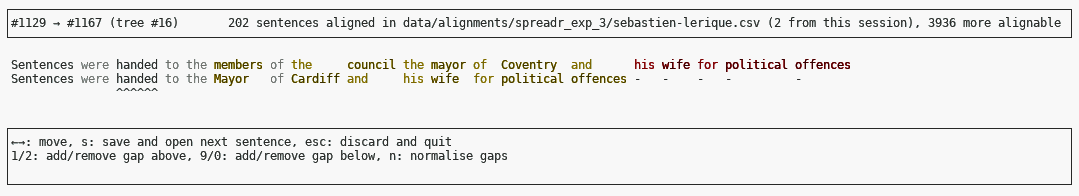
\includegraphics[width=\linewidth]{images/manual/gistr-goldcli-before.png}
  }

  \subfloat[After manual alignment]{
    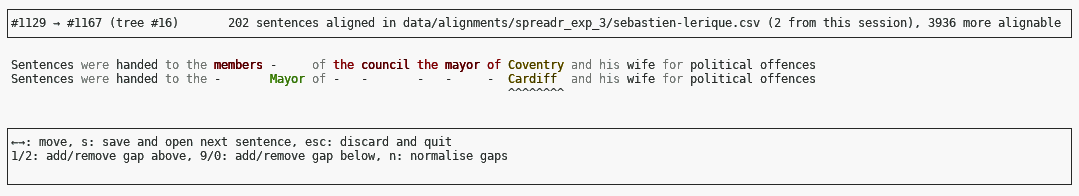
\includegraphics[width=\linewidth]{images/manual/gistr-goldcli-after.png}
  }
  \caption[Console interface for manual transformation alignment]{
  \textbf{Console interface for manual transformation alignment.}
  The user moves their cursor (underline below "handed" and "Cardiff") along the word sequences to insert or remove gaps and align the two utterances by hand.
  }
  \label{fig:gistr-goldcli}
\end{figure*}

Finally, we manually evaluated the overall quality of these parameters
by hand-coding the number of errors in a random set of 100 non-trivial
alignments generated by the parameters. Errors were counted as the
number of words whose alignment would have to be changed in order to
obtain a perfect alignment. Of those 100 alignments, 79 were perfect, 12
had 1 error, 4 had 2 errors, and the remaining 5 had between 3 and 6
errors. Counting 1 error as acceptable, this method yields a successful
alignment in 91\% percent of the cases. To make sure this is also the
case for deep alignments, we hand-coded errors in 100 random alignments
for which the algorithm had explored exchanges (though not all of them
are deep alignments, as it may be that the shallow alignment was the
best). An error was counted for each exchange that was missing,
mistaken, or should not have been present at all. Of the 100 alignments,
81 had no errors, 17 had 1, and 2 had 2 errors. The parameters obtained
here were thus used for all further analyses. They are also the ones
used in the example alignments discussed in the previous sections.

\subsection{Transformation model}\label{transformation-model}

The alignment procedure we just presented provides a list of deep
alignment trees for each transformation in the data set. At this point
we have showed that such deep alignments reliably encode the details of
a transformation broken down into smaller operations, thus completing
the first step of our modelling approach. We now proceed to the next
step: first, create an accurate visualisation of the details of
transformations captured by the alignments, then derive a transformation
model based on that visualisation. The step after that will then refine
the model and quantify the behaviours we can measure with it.

\subsubsection{Consensus filiations}\label{consensus-filiations}

The first step to visualise the process encoded by alignments is to
reduce the possibly multiple deep alignments encoding a transformation
into a single version, which we call the consensus alignment. Indeed for
a given transformation \(u \rightarrow u'\), a word in \(u\) could for
instance be assigned to different words in \(u'\) for different choices
of deep alignments. Other cases are possible, as \(w\) could be deleted
in one deep alignment and not in others, and so on and so forth. A
method to resolve conflicts across multiple deep alignments is therefore
required.

We adopt the following procedure to construct the consensus alignment
from the list of deep alignment trees of a transformation
\(u \rightarrow u'\). First, flatten each deep alignment tree into a
list. Recall that in a tree of deep alignments, a path from the root to
a leaf uniquely corresponds to one of the deep alignments encoded in the
tree: each tree encodes as many deep alignments as it has leaves. This
step thus takes each tree, and turns it into the list of deep alignments
that it encodes. Then, concatenate all the lists together. We are thus
left with a list of uniquely defined deep alignments for the
transformation. For instance, if we had \(n\) deep alignment trees with
\(m_1\), \ldots{}, \(m_n\) leaves in each tree, we now have a list of
\(m_1 + ... + m_n\) uniquely defined deep alignments.

Given this list of deep alignments, we then examine which operations are
present in the majority of the deep alignments. More precisely, for a
given word \(w\) in \(u\), determine if it is conserved either exactly
or through replacement in at least half of all the deep alignments. if
it is, then select the child word in \(u'\) which appears in most deep
alignments (i.e.~the majority child); if \(w\) is not conserved in at
least half of the deep alignments, then consider it deleted. Any word in
\(u'\) that has no assigned parent word is then considered an insertion.

A few details are worth mentioning here. First, a word that is stable in
exactly half the deep alignments and deleted in the other half is still
considered stable, such that the procedure sometimes maintains one or
two more stable words than the deep alignments it synthesises. Such
conflicts are inherent to any consensus method, and the alternative in
this case would be to consider the word unstable, adding deletions and
insertions instead of stabilities to the consensus alignment; we choose
to favour stabilities so as not to inflate operations artificially.
Second, an analogous conflict can arise when a stable word has two
equally probable candidate children, or conversely a given child word
has two equally probable parent words. In those cases we decide in
favour of the word closest to the end of the utterance, and the
procedure is consistent in both directions: the consensus alignment for
\(u \rightarrow u'\) is the same as for \(u' \rightarrow u\). Finally, a
small number of cases create new single-word exchanges, as two words are
assigned not the same child but different children at exchanged
positions; manual inspection of these cases showed that such exchanges
are consistent with the transformation they represent. In practice, only
53 of the 3461 transformations in Experiment 3 have more than one deep
alignment, 46 of which have 2 (the other seven having 3 to 6 deep
alignments), such that any change here has virtually no impact on the
results.

Now, consider for instance a simple branch
\(u \rightarrow u' \rightarrow u''\). A word \(w'\) in the middle
utterance \(u'\) is now uniquely identified (by the consensus alignment)
either as an insertion, or as the conservation or replacement of a
parent word \(w \in u\) (with or without movement due to an exchange).
Continuing down the branch, \(w'\) can also be linked to its child
\(w''\) (if it was not deleted), thus creating a lineage for this
specific word along the branch. Constructing consensus alignments for
each transformation thus allows us to follow the ancestry and descent of
individual words through parent and child transformations in a branch.

\subsubsection{Branch and utterance
dimensions}\label{branch-and-utterance-dimensions}

\Cref{fig:gistr-lineage-tree} represents the lineages produced by this
procedure on the branches of an example tree taken from Experiment 3,
whose root is the following utterance:\footnote{This is tree \#4, which
  is also shown in \cref{fig:gistr-trees}. The transition from depth 1
  to depth 2 in branch \#49 of the figure also corresponds to the
  transformation of utterance \ref{ut:49} to utterance \ref{ut:120}
  discussed when introducing deep alignments.}

\begin{nquote} % <!-- #4 -->
  « At Dover, the finale of the bailiffs' convention. Their duties, said a speaker, are "delicate, dangerous, and insufficiently compensated." »
\end{nquote}

\begin{figure*}[!h]
  \centering
  \includegraphics[width=\linewidth]{images/computed/exp_3/lineage-tree-4.png}
  \caption[Example lineages for all the branches of tree \#4 from Experiment 3]{
  \textbf{Example lineages for all the branches of tree \#4 from Experiment 3.}
  Each subplot corresponds to a different branch.
  The horizontal axis is the depth in the branch, and the vertical axis is the index of each word in its utterance.
  A grey line represents a word lineage along the branch, and the darkness of the line corresponds to the length of the path between the word's first appearance (or the branch start) and its disappearance (or the branch end);
  darker lines thus represent words that last longer across transformations (since branches eventually stop, however, our view of the process is truncated and the darkness is less reliable for words that appear towards the end of a branch).
  At each depth, the darker background band indicates what the subject sees, and the lighter band indicates the transformation that the subject made.
  Inside lighter bands:
  red dots are word deletions, green dots are word insertions, blue dots are word replacements, and exchanges can be seen when bundles of lines cross each other.
  Dots inside each light band are spread out on the horizontal axis so as make them easier to distinguish visually, but the horizontal position of a dot inside its band has no further meaning.
  }
  \label{fig:gistr-lineage-tree}
\end{figure*}

At first glance the plots reflect the rapid shortening of utterances,
and the fact that transformations are less important on shorter
utterances deeper in the branches. The figure also indicates that word
replacements, studied in the previous chapter with data from blogspace,
are quite speckled: they are less frequent than deletions and
insertions, and affect smaller portions of the utterances when they
appear. As replacements were the only process that could be extracted
from the blogspace data set, suspecting this caveat was one of the
motivations for our current experimental approach.

The plots also show noticeable regularities in the way transformations
vary. To discuss these we distinguish between the two axes of
\cref{fig:gistr-lineage-tree} as two scales of the representation, each
of which corresponds to a different set of events. First the horizontal
axis: an event at this level is the bulk transformation or conservation
of an utterance by a subject, without going into the detail of the way
an utterance changes. This yields a series of conservation and
transformation events, one at each depth in the branch. Call this the
branch dimension, pictured in \cref{fig:gistr-dimensions-branch}. A
salient feature on this dimension is the apparent burstiness of
transformations. Since successive subjects perform transformations
independently, confirming this trend would indicate a behaviour in
utterance evolution reminiscent of punctuated equilibria: a
transformation occurring after a period of stability would result in a
new utterance that is more likely to be transformed again. We quantify
this trend further down.

Second, the vertical axis which delves into the detail of a
transformation represented as a set of word insertions, deletions,
conservations and replacements with or without exchange. Call this the
utterance dimension. An important feature of this representation of
transformations is its uniqueness. Indeed, at the mathematical level a
consensus alignment encodes a transformation as a pair of word sequences
with gaps (and possible sub-alignments of exchanged parts), an encoding
that is not unique. Insertions and deletions that happen together can be
reordered (putting insertions before their neighbouring deletions
instead of the other way around, or alternating an insertion with a
deletion). The exchange of two parts around a stable chunk can also be
re-encoded by inverting the roles of stable and exchanged chunks, all
without changing the transformation represented by the encoding. By
compressing the gaps in this encoding, the utterance dimension merges
these equivalent versions together and produces a unique diagram
representing the transformation. We picture this correspondence between
the transformation diagram in the utterance dimension and the compressed
form of consensus alignments in \cref{fig:gistr-dimensions-utterance}.

\begin{figure*}[!h]
  \centering
  \subfloat[\textbf{Branch dimension.}
  This level looks at whether or not an utterance is transformed, without going into the detail of changes (hence the greyed out dots and lines).
  Similar to Fig.~\ref{fig:gistr-lineage-tree}, light grey bands are what subjects see, and the bands between those represent what the subjects do with what they read.
  An orange band indicates that an utterance was transformed, that is a T event, and a dark grey band indicates that an utterance was perfectly conserved, that is a C event.
  The corresponding ordered series of events is shown underneath the axis' arrow.]{
    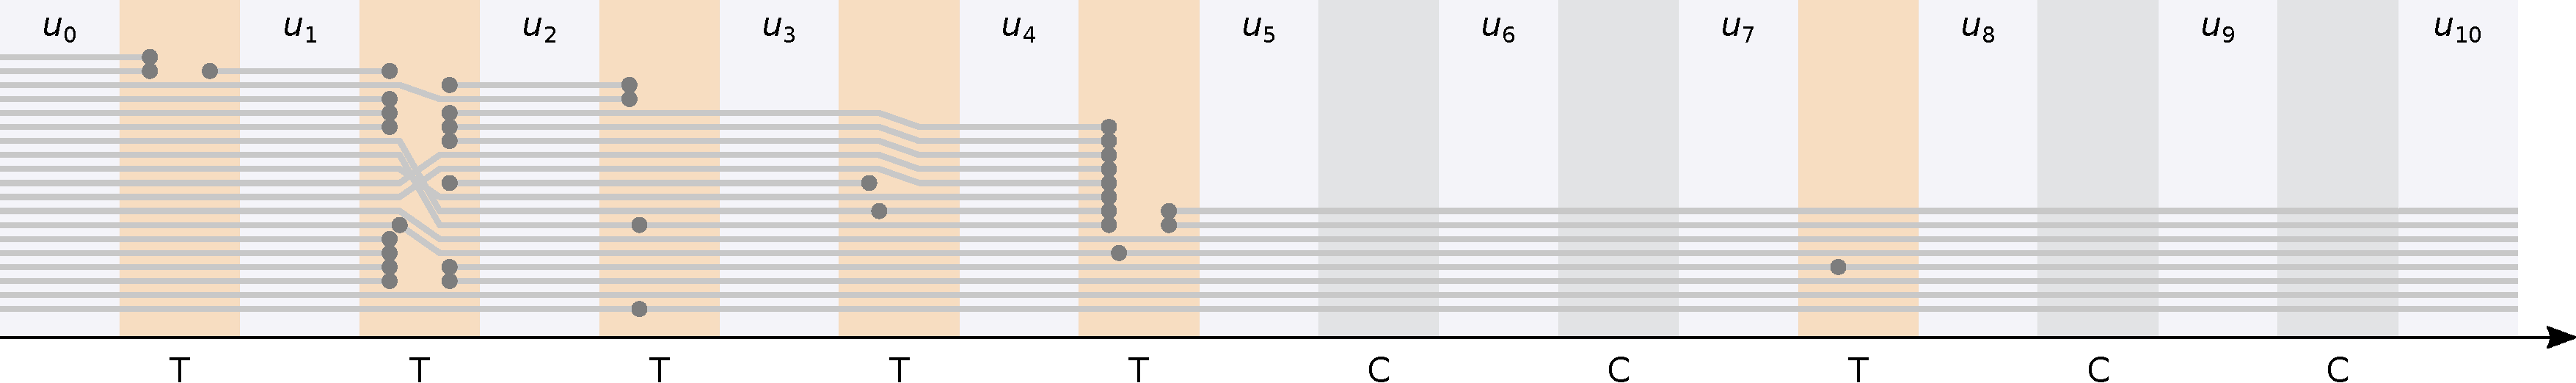
\includegraphics[width=\linewidth]{images/manual/gistr-dimensions-branch.pdf}
    \label{fig:gistr-dimensions-branch}
  }

  \subfloat[\textbf{Utterance dimension.}
  This level looks at the detail of a transformation, and represents it with a diagram that compresses the pair of sequences produced by aligning parent and child utterances.
  This diagram uniquely represents the transformation, and merges any variations in encoding that can exist in pairs of sequences with gaps.
  The top level of the figure shows how the canonical representation comes from the lineage plots.
  The bottom level shows two equivalent encodings of the same transformation (as would be produced by the alignment tool), which compress to the same canonical representation.]{
    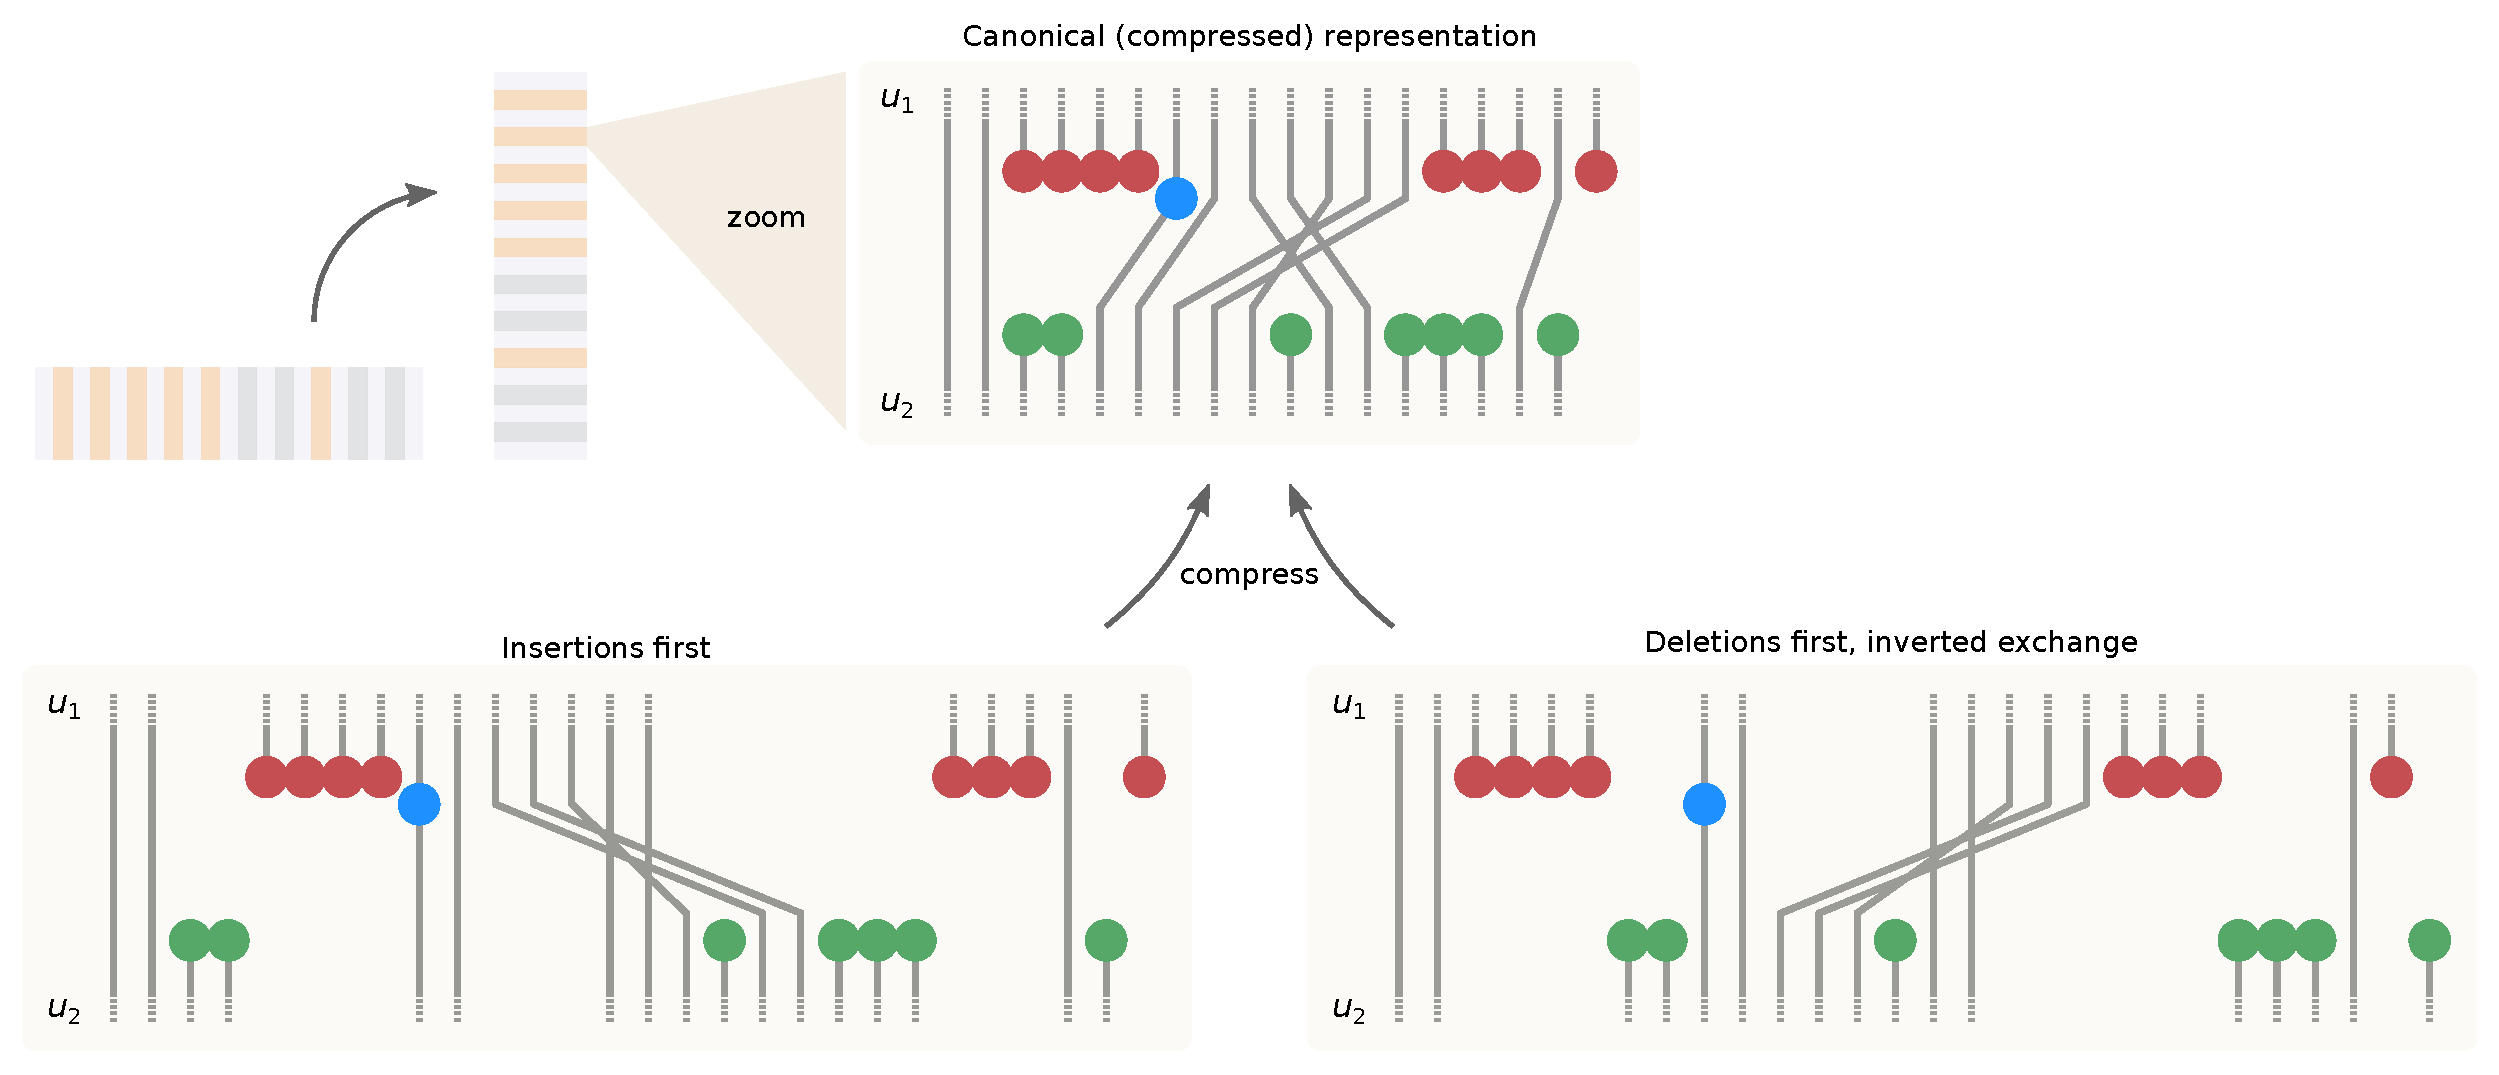
\includegraphics[width=\linewidth]{images/manual/gistr-dimensions-utterance.pdf}
    \label{fig:gistr-dimensions-utterance}
  }

  \subfloat[\textbf{Parent and child arrays of operations.}
  The canonical representation is further simplified by discarding the change in position encoded by word exchanges, and only keeping the information on whether a word is conserved or replaced.
  The procedure results in two arrays of word operations:
  a parent array made of conservations (C), replacements (R) and deletions (D), and a child array made of conservations, replacements and insertions (I).
  Conservations and replacements in the parent array, if not involved in exchanges, are linked to their corresponding operation in the child array, such that we can compute the distance between a block of insertions in the child and a block of deletions in the parent (except when exchanges separated the blocks).]{
    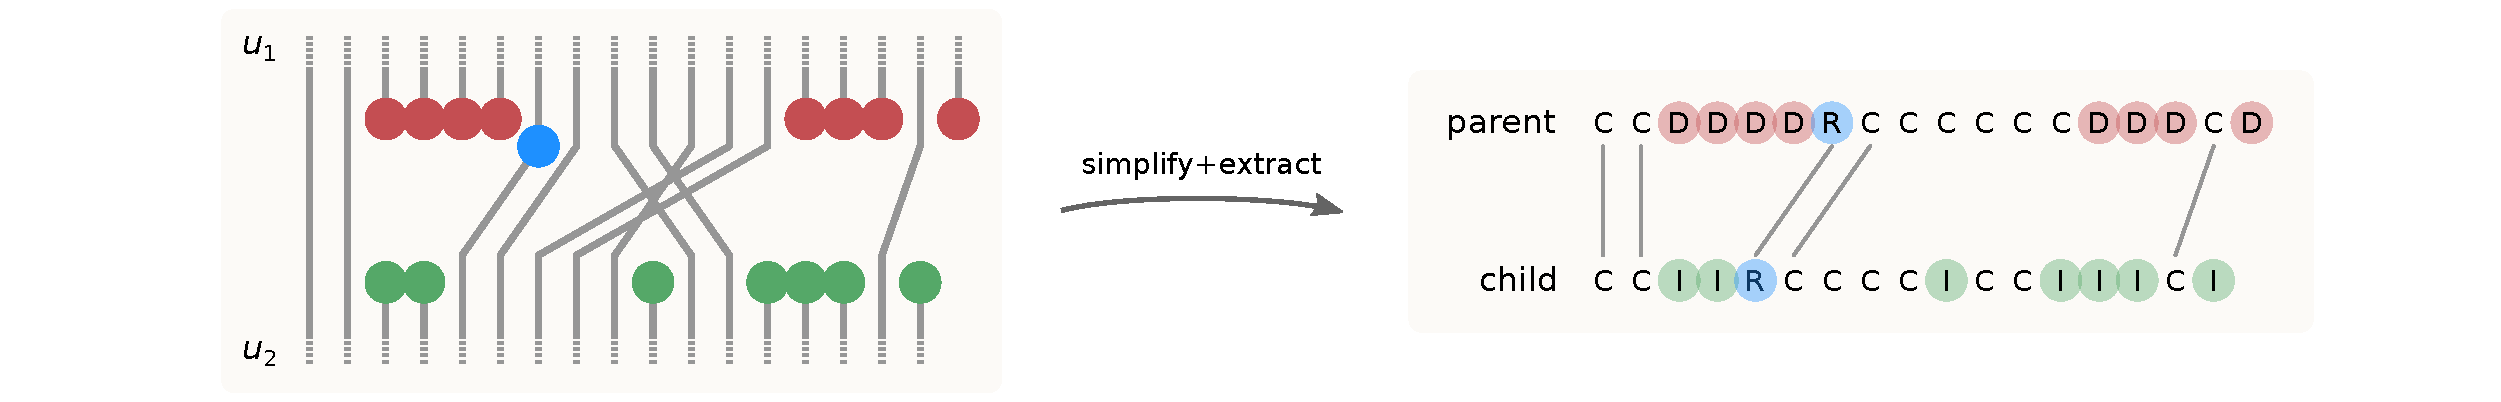
\includegraphics[width=\linewidth]{images/manual/gistr-utterance-arrays.pdf}
    \label{fig:gistr-utterance-arrays}
  }
  \caption[Analysis dimensions]{
  \textbf{Analysis dimensions.}
  Transformations are analysed along two dimensions.
  The branch dimension only looks at whether utterances are transformed or not, thus sees a series of T (transformed) and C (conserved) events.
  The utterance level looks at the detail of the transformations, and after simplification represents them with two arrays of operations, one for the parent utterance (made of C, R and D operations) and one for the child utterance (made of C, R and I operations).
  This example is built on branch \#49 from Fig.~\ref{fig:gistr-lineage-tree}.
  }
  \label{fig:gistr-dimensions}
\end{figure*}

This subtlety in the encoding of transformations is not a coincidence.
It relates to the fact that, in spite of the one-dimensional nature of
text written on a line, utterance transformation is a multi-level
process that can operate on whole groups of words at a time (for
instance when insertions and deletions happen together) and does not
necessarily reduce to a sequential series of events. Manually inspecting
the branches' transformations on the utterance dimension indicated
several trends to that effect, several of which are visible in
\cref{fig:gistr-lineage-tree}:

\begin{itemize}
\item
  Deletions, exchanges, and insertions seem bursty, that is they appear
  in large chunks (a behaviour that replacements do not seem to have).
  The bursts also seem longer if the utterance they appear in is longer.
\item
  Insertions seem to rarely occur without deletions. When they appear
  with deletions, the two tend to be close to each other and of similar
  magnitude.
\item
  All operations are less frequent at the very beginning of utterances.
\end{itemize}

As we just noted, burstiness at the word level is no surprise: words are
not processed independently and transforming parts of an utterance is
likely to depend on syntactic and semantic boundaries. However, the
behaviour of the bursts imposes constraints on the kind of model that
can account for the transformation process. In particular, the fact that
insertions and deletions seem to be of similar magnitude when close to
each other is not easy to account for. For instance, when creating an
insertion, a generative model must be aware of any deletions that have
already been created in the vicinity, and take their size into account.
Such a generative model would need to involve memory and attention span
mechanisms that allow bursts to relate to their neighbouring operations
(both preceding and following). Similarly, accounting for exchanges with
a generative model also requires at least a memory component that is
capable of recalling the postponed part of an exchange. Such mechanisms
are beyond the score of this chapter, and we therefore focus on
developing a descriptive---rather than generative---model. While it will
not allow for a reconstruction of the transformation process, this
approach will provide a synthetic understanding of the transformation
behaviour without needing to rely on cognitive mechanisms. By
abstracting out the basic building blocks of transformations, we will
then be able to gradually increase the level of detail with which we
understand the regularities of their interactions.

\subsubsection{Descriptive transformation
model}\label{descriptive-transformation-model}

Our model relies on a simplification of the transformation diagrams in
the utterance dimension of lineage plots, which we take to be the
canonical representation of a transformation. In order to keep the model
palatable, we first set aside part of the information provided by
exchanges. Indeed, the natural way of analysing an exchange in a
transformation diagram is to see it as a permutation of a sub-sequence
of words in the utterance, with possible replacements, insertions and
deletions added in-between. Analysing the regularities of such a process
is matter for a model in itself, and we chose to leave this aspect of
transformations for further research. We instead focus on insertions,
deletions and replacements only. When words are exchanged we consider
only whether they are replaced or conserved, and do not look at their
change of position. Note that while this excludes any shifts in position
from our model, the approach still benefits from having detected
exchanges earlier in the procedure: it guarantees that the remaining
insertions and deletions correspond to actual appearances and
disappearances, not undetected exchanges.

From a given transformation diagram we then extract two arrays of
word-level operations,\footnote{We use the phrase \enquote{array of
  operations}, and not \enquote{series of events}, to emphasise that
  these operations exist on the one-dimensional utterance axis, but do
  not necessarily come from a sequential generation process. The two
  terms refer to the same mathematical object, and simply change the
  interpretation of the index: for a series of events the index
  represents time, for an array of operations it does not.} one for the
parent utterance and one for the child utterance. Parent and child
arrays both may contain conservation and replacement operations, and
parent arrays may contain deletion operations while child arrays may
contain insertion operations. The transformation diagram further
provides us with the correspondence of conservation and replacement
operations between the two arrays (except for operations that were
involved in an exchange, for which we lose position information), such
that we can measure the distance between two blocks of insertions and
deletions (except if the two blocks are separated by operations involved
in an exchange).

\Cref{fig:gistr-utterance-arrays} illustrates this simplification of
transformations, which we use as our model for the process: it
represents a transformation as two arrays of word-level operations, one
for the parent utterance made of word conservations, replacements, and
deletions, and one for the child utterance made of word conservations,
replacements, and insertions. Some operations happen on several
contiguous words at a time, and we call these \emph{chunk-level
operations}. Conversely, when referring to operations defined as single
word insertions, deletions, replacements or conservations, we will use
the phrase \emph{word-level operation}, or simply \emph{operation} when
the context is clear. Contiguous word-level operations, then, form a
single chunk-level operation.

Note that a word-level conservation or replacement in one array can
additionally, but not necessarily, be paired with another word-level
conservation or replacement in the other array. Thus, when chunk-level
insertions and deletions are separated by paired conservations or
replacements, we define the distance between the two chunk-level
operations as the number of conservations or replacements separating the
two. For instance, a chunk-level insertion can appear two words after a
chunk-level deletion, and this information will be useful when comparing
the sizes of chunk-level insertions and deletions in a given
transformation. When unpaired conservations or replacements separate
chunk-level insertions and deletions, however, this distance will remain
undefined.

\subsection{Model refinement}\label{sec:gistr-results-inner}

Having defined our model for transformations, we now delve into the
detailed behaviour that it captures. We do so in three stages. First, we
quantify the extent to which transformations are bursty, both in the
branch dimension and in the detailed transformation model (utterance
dimension). In doing so we establish the prevalence of chunk-level
operations in the transformation model. We then characterise the number
of word-level and chunk-level operations that occur in utterances,
linking their magnitude and probability to the length of the parent
utterance and the position at which they occur. Finally, we examine the
dependencies between each operation type, and highlight a close
relationship between insertions and deletions.

\subsubsection{Bursty behaviours}\label{bursty-behaviours}

We begin by measuring the extent to which each dimension features bursty
behaviour. Following \textcite{jo_circadian_2012}, who rely on
\textcite{goh_burstiness_2008}, we measure the burstiness of a series of
events through the parameter \(B\) defined as

\[B = \frac{\sigma_{intervals} - \mu_{intervals}}{\sigma_{intervals} + \mu_{intervals}}\]

where \(\sigma_{intervals}\) and \(\mu_{intervals}\) are respectively
the standard deviation and mean of the distribution of inter-event times
in the series of events. The same computation applies to arrays of
operations (the two have the same mathematical description). \(B\) has
values between -1 and 1; \(B = -1\) corresponds to a perfectly regular
process (\(\sigma_{intervals} = 0\), and \(\mu_{intervals} > 0\) is the
constant period of events), \(B = 0\) indicates a burstiness similar to
that of a Poisson process, where the occurrence of a new event does not
depend on the presence of previous events (and
\(\sigma_{intervals} = \mu_{intervals}\)), and \(B = 1\) corresponds to
an asymptotically perfectly bursty process (it is the limit
\(\sfrac{\mu_{intervals}}{\sigma_{intervals}} \rightarrow 0\)).
Intuitively, a process with average inter-event time shorter than its
standard deviation will often have events close to each other with a few
long intervals without events, and a process with an average inter-event
time longer than its standard deviation will have events more evenly
spaced relative to their mean spacing.

Note that this measure can be applied to any series of events, and we
therefore use it in both the utterance and the branch dimensions. In the
utterance dimension, it tells us the extent to which the changes that a
subject makes in an utterance tend to occur in contiguous chunks. We
will see that this chunkiness is very strong, so much that we will start
examining insertions and deletions and the level of chunks. In the
branch dimension, the measure tells us how bursty the evolution along a
branch is. A bursty evolution would indicate a punctuated equilibria
behaviour, with long periods of stability interrupted by sudden bursts
of transformations. A non-bursty behaviour would indicate that a
subject's transformations do not influence the following subject so
much.

Let us start with the utterance dimension. In the parent array, we note
the series of deletion events \(\mathcal{D}\) and the series of
replacements \(\mathcal{R}_p\). In the child array, we note the series
of insertion events \(\mathcal{I}\) and the series of replacements
\(\mathcal{R}_c\). A conserved word is considered an absence of event.
Note that because of inserted and deleted words, replacements may not
appear with the same distributions in the parent and child arrays. As a
consequence, \(\mathcal{R}_p\) and \(\mathcal{R}_c\) may not have the
same distribution of inter-event times. The burstiness measures for each
of these series are shown in
\cref{fig:gistr-utterance-burstiness-words}, along with the burstiness
of the series made of all parent or child events without distinguishing
their type. The plots show that deletions and insertions are both
bursty, while replacements are undistinguishable from a non-bursty
process such as a Poisson process. When all event types are joined
together, the process is also bursty, albeit slightly less.

Given the strength of this behaviour for deletions and insertions, we
further look at these series by collapsing each contiguous set of
deleted or inserted words into a single event. This leads to a series of
chunk-level deletions and insertions separated by word-level
replacements and conservations (non-events). For inter-event times, this
corresponds to removing the null values in the previous distributions of
inter-event times (which separated words in the same chunk-level
operation); computing the burstiness of the chunk-level process is
therefore straightforward. The values plotted in
\cref{fig:gistr-utterance-burstiness-chunks} show that none of the
chunk-level processes are bursty; rather, they are slightly more regular
than a Poisson process would be.

\begin{figure}[!ht]
  \centering
  \subfloat[Burstiness of word-level operations]{
    \includegraphics[width=.55\linewidth]{images/computed/exp_3/burstiness-words.png}
    \label{fig:gistr-utterance-burstiness-words}
  }
  ~
  \subfloat[Burstiness of chunk-level operations]{
    \includegraphics[width=.40\linewidth]{images/computed/exp_3/burstiness-chunks.png}
    \label{fig:gistr-utterance-burstiness-chunks}
  }
  \caption[Burstiness of operations in the utterance dimension]{
  \textbf{Burstiness of operations in the utterance dimension.}
  The left pane shows the burstiness of each type of word-level operation in parent and child arrays, as well as the burstiness of the series made of all operations joined regardless of their type.
  The right pane shows the burstiness for deletions, insertions, and joined events, where contiguous sets of operations are collapsed into single events.
  This corresponds to the burstiness of chunk-level deletions, insertions, and joined events.
  Grey lines are the 95\% confidence intervals based on Student's $t$-distribution, considering each tree as an independent burstiness measure.
  }
  \label{fig:gistr-utterance-burstiness}
\end{figure}

Although this behaviour is consistent with our intuition of the way an
utterance is reformulated, there is a question as to whether the
alignment procedure does not favour burstiness. Indeed, the scores of
operations are parametrised in such a way that insertion and deletion
gaps are assigned different costs for initial opening and extension.
However, while this parametrisation makes it possible for burstiness to
be more easily identified, it does not make it a necessity: setting the
gap opening cost to the same value as the gap extension cost would make
the alignment tool neutral with respect to burstiness (setting it lower
would be biased against burstiness, and the alignment algorithm would
favour word mismatches over gaps to encode differences). In our case,
the parameters we trained set the gap opening cost to a much higher
value than the extension cost (.29 vs. .12 in absolute values), such
that the alignment tool does find bursty insertions and deletions more
easily. However, these parameters are learned from hand-coded alignments
and their output has been validated on test samples: any bursty
insertions or deletions detected by the alignments is therefore the
product of the data itself, and not an artefact.

Let us now step back and look at the evolution along the branches, that
is, the branch dimension. We ask whether the fact that an utterance is
transformed has an effect on the subsequent transformations by other
subjects. Here the situation involves only one event type: the
transformation of an utterance is an event, and the conservation of an
utterance is the absence of an event. Note that our data in this
dimension is truncated due to branches not being infinite. When the last
subject in a branch does not transform the utterance they reproduce, we
do not observe the actual duration of that stability: had the branch
continued, the stability could have been interrupted immediately, or
could have lasted for many more reproductions of the utterance.
Including these truncated intervals in the distribution of inter-event
times artificially inflates the burstiness (because it adds
underestimated intervals to the distribution), but removing them biases
our sample towards inter-event times for longer utterances (earlier in
the branch), which could also inflate burstiness. We thus present
measures for both distributions, with and without the truncated
intervals.

Burstiness in the branch dimension with truncated intervals is
\(B_{branch,all} = 0.252 \pm 0.029\), and burstiness without the
truncated intervals is \(B_{branch,observed} = 0.304 \pm 0.031\) (both
error estimates correspond to the 95\% confidence interval based on
Student's \(t\)-distribution, considering each tree as an independent
burstiness measure). Both measures show that the transformation process
in the branch dimension is significantly bursty. This is consistent with
our intuition that when a transformation appears after a period of
stability, it is likely to trigger other transformations following it
until a new stable (often much shorter) utterance is reached.

\bigskip
Overall, it appears that insertions and deletions inside an utterance
tend to cluster into chunks, which is not a surprise as sentence
processing does not happen at the word-level only. Still, this makes the
chunk-level of analysis relevant for what follows. Replacements,
conversely, do not appear in chunks, and chunk-level operations
themselves also do not cluster into higher-kinded chunks. Interestingly,
the evolution along branches is also bursty, although this is due to an
entirely different process: the measure suggests that when one subject
transforms a previously stable utterance, the new production is itself
more susceptible to further transformations that could be regularising
the changes introduced by the first subject.

\subsubsection{Position and utterance
length}\label{position-and-utterance-length}

The general trends presented in \cref{sec:gistr-results-general}
indicated that utterance length has a strong effect on the probability
and magnitude of transformations. The transformation models now lets us
explore in detail the way word-level and chunk-level operations depend
on the size of an utterance, on one side, and on the position at which
they occur, on the other.

We begin by looking at the probability of each operation as a function
of utterance length. \Cref{fig:gistr-ops-prob} plots the logistic
regression of the presence or absence of deletions, insertions, and
replacements as a function of the number of words in the parent
utterance. The length of the parent utterance has a significant effect
on all three operations, with deletions being the quickest to increase
in probability, followed by replacements then insertions: the threshold
for having deletions over half the time is 19 words, 22.6 for
replacements, and 28.1 words for insertions; the slopes of the
regressions are also ordered this way. In other words, a longer
utterance will have a higher risk for all operations, and the increase
is strongest for deletions, then for replacements, then for insertions.

\Cref{fig:gistr-ops-count} further shows the number of operations as a
function of parent utterance length, either counting one for each
word-level operation or counting one for each chunk-level operation. The
number of word-level and chunk-level operations increase close to
linearly as a function of parent length. Deletions have by far the
strongest link to parent length, both at the word and chunk levels,
followed by insertions then replacements. Note that the replacement
counts barely change between word and chunk level since this operation
is not bursty: it affects mostly isolated words instead of contiguous
sets of words. In short, a longer utterance has a higher probability of
suffering any type of operation, with on average over a quarter of the
words deleted, the equivalent of a fourteenth of the original utterance
in new words, and about a twentieth of the words replaced.

\begin{figure}[!ht]
  \centering
  \subfloat[\textbf{Probability of word operations w.r.t. parent length.}
  Computed as the log-odds logistic regression of the presence or absence of a given operation in the transformation of $u_p$ (parent) into $u_c$ (child), versus the number of words in $u_p$.
  Colours correspond to the colour-coding used in Fig.~\ref{fig:gistr-lineage-tree}.
  Light shades are 95\% regression confidence intervals.]{
    \includegraphics[width=\linewidth]{images/computed/exp_3/p-ops_parent-length_logistic.png}
    \label{fig:gistr-ops-prob}
  }

  \subfloat[\textbf{Number of word-level and chunk-level operations w.r.t. parent length.}
  Parent lengths are binned into 5 quantile-based bins.
  The word-level counts the number of individual words affected by an operation (deletion, insertion, replacement).
  The chunk-level counts the number of contiguous sets of words affected by an operation.
  Light shades are 95\% regression confidence intervals, and vertical bars are 95\% confidence intervals for the value of a bin (Student $t$-based, here counting each operation as an independent measure).
  % \todo{FIXME: vertical bars should count each transformation as independent}
  ]{
    \includegraphics[width=\linewidth]{images/computed/exp_3/chunk-size_parent-length.png}
    \label{fig:gistr-ops-count}
  }
  \caption[Probability and number of word-level or chunk-level operations]{
  \textbf{Probability and number of word-level or chunk-level operations.}
  }
  \label{fig:gistr-ops-counts}
\end{figure}

Manual exploration of the lineage plots also indicated that operations
are not positioned evenly in the utterances. To quantify this behaviour
we apply the susceptibility measure developed in the previous chapter to
positions in an utterance. For words at position \(x \in [0, 1]\)
relative to their utterance's length (\(x = 0\) for words at the
beginning, \(x = 1\) for words at the end), the susceptibility
\(\sigma_O(x)\) to an operation \(O \in \{D, I, R\}\) is defined as the
ratio of \(s_O(x)\), the number of times words at relative position
\(x\) are the target of operation \(O\), to \(s_O^0(x)\), the number of
times those words would be the target of operation \(O\) if the choice
of words were random:\footnote{Since operations in a given
  transformation are not independent, we scale both \(s_O(x)\) and
  \(s_O^0(x)\) such that each transformation has a maximum contribution
  of 1 to the total counts. This procedure is similar to the
  susceptibility scaling approach we followed in the previous chapter.}

\[\sigma_O(x) = \frac{s_O(x)}{s_O^0(x)}\]

\Cref{fig:gistr-susc-ops} plots \(\sigma_D\), \(\sigma_I\) and
\(\sigma_R\) (for replacements on the parent side) both overall and for
binned parent lengths. The leftmost plots show that deletions and
insertions are half as likely to appear at the very beginning of an
utterance as they would at random, and more likely than random in the
second half of an utterance. This is consistent with the well-known
primacy effect in recall of word lists. In this case, subjects transform
the beginning of an utterance on average much less than the rest.
Replacements feature this primacy effect to a lesser extent, with the
addition of a slight recency effect: words at the end of an utterance
are slightly less replaced than non-extremity words. The plots at binned
parent lengths show little to no variation in these patterns: each
pattern is more or less marked depending on the parent sentence length
(especially for replacements, which seem more uniform for short
utterances), but the general behaviour is the same for different parent
lengths.

\begin{figure}[!ht]
  \centering
  \subfloat[Deletions]{
    \includegraphics[width=\linewidth]{images/computed/exp_3/susceptibility-del_position_parent-length.png}
    \label{fig:gistr-susc-del}
  }

  \subfloat[Insertions]{
    \includegraphics[width=\linewidth]{images/computed/exp_3/susceptibility-ins_position_parent-length.png}
    \label{fig:gistr-susc-ins}
  }

  \subfloat[Replacements]{
    \includegraphics[width=\linewidth]{images/computed/exp_3/susceptibility-rpl_parent_position_parent-length.png}
    \label{fig:gistr-susc-rpl}
  }
  \caption[Susceptibility for word operations as a function of relative position in the utterance]{
  \textbf{Susceptibility for word operations as a function of relative position in the utterance.}
  The leftmost plot of each sub-figure (blue background) shows $\sigma$ computed over all transformations.
  The plots with the white backgrounds show $\sigma$ computed over transformations with binned parent utterance lengths, indicated in the plot titles.
  Parent length bins are quantile-based, that is computed to have the same number of utterances in each bin (the bins are identical to Fig.~\ref{fig:gistr-ops-count}).
  Light shades are the 95\% confidence intervals computed following the \textcite{goodman_simultaneous_1965} method for multinomial proportions, considering each transformation as an independent measure.
  }
  \label{fig:gistr-susc-ops}
\end{figure}

Finally, we examine the dependence of chunk-level operation size on its
position in an utterance. The manual exploration of lineage plots did
not hint to any effect at this level, but the question now appears
legitimate: since subjects delete words on average more often towards
the end of an utterance, it is possible that those deletions are also
longer if they correspond to larger memory loss.
\Cref{fig:gistr-chunk-size} shows the dependence of chunk-level
operation size on position in the utterance, for deletions, insertions
and replacements, both overall and for binned parent length. Deletions
exhibit a slight effect of position on chunk-level operation size, which
is significant for parent lengths between 11 and 15 words.\footnote{The
  plots also indicate that the overall chunk-level operation size
  increases with parent length, a slight effect which was confirmed for
  deletions and insertions with dedicated regressions, but which we do
  not discuss further given its mildness (slopes respectively .030 and
  .013, both significative with \(p < .001\)).} That is, for those
lengths, deletions towards the end of the utterance are significantly
larger than deletions at the beginning (4.1 words versus 1.7 words on
average), in addition to being more frequent (see the susceptibility
plots above). The trend is present for deletions at all lengths, though
most of the time not significative. Other operations do not seem to
exhibit this behaviour (the variations for insertions are not
significative).

\begin{figure}[!ht]
  \centering
  \includegraphics[width=\linewidth]{images/computed/exp_3/chunk-size_position_parent-length.png}
  \caption[Chunk-level operation size w.r.t. parent length and position in utterance]{
  \textbf{Chunk-level operation size w.r.t. parent length and position in utterance.}
  The leftmost plot (blue background) shows the average chunk-level operation size w.r.t. parent length for all utterances.
  The plots on its right (white background) divide that data into binned parent lengths (bins identical to Figs.~\ref{fig:gistr-ops-count}--\ref{fig:gistr-susc-ops}).
  In each plot, the height of a line for a given relative position $x$ corresponds to the average size of the chunk-level operations in which words at position $x$ are found;
  for instance, a chunk-level deletion that spans the second half of an utterance will be spread over $x \in [.5, 1]$.
  Average sizes are weighted such that each utterance contributes 1 unit.
  Light shades are the 95\% confidence intervals (Student $t$-based, considering each transformation as an independent measure).
  }
  \label{fig:gistr-chunk-size}
\end{figure}

Overall, these measures show that deletions are more frequent than
insertions, which are more frequent than replacements. Operations happen
preferentially in the second half of utterances (except replacements
which favour all positions except extremities), and the number of
word-level and chunk-level operations are proportional to the parent
length. Chunk-level deletions are also larger in the second half of
utterances, compared to in the first half.

\subsubsection{Dependencies between
operations}\label{dependencies-between-operations}

Manual exploration of the lineage plots indicated that operations have
non-trivial dependencies between each other. The contingency table
combining the presence or absence of each operation gives an overview of
these dependencies:

\begin{center}
  \begin{tabular}{llrrrr}
    \toprule
     & & \multicolumn{4}{c}{\textbf{Deletion}} \\
    \cmidrule(l){3-6}
     & & \multicolumn{2}{c}{\emph{no}} & \multicolumn{2}{c}{\emph{yes}} \\
    \cmidrule(lr){3-4} \cmidrule(l){5-6}
    \multicolumn{2}{l}{\textbf{Replacement}} & \multicolumn{1}{c}{\emph{no}} & \multicolumn{1}{c}{\emph{yes}} & \multicolumn{1}{c}{\emph{no}} & \multicolumn{1}{c}{\emph{yes}} \\
    \midrule
    \multirow{2}{*}{\textbf{Insertion}} & \emph{no} & 1381 & 415 & 286 & 308 \\
     & \emph{yes} & 66 & 94 & 399 & 512 \\
    \bottomrule
  \end{tabular}
\end{center}

\begin{figure}[!ht]
  \centering
  \includegraphics[width=.6\linewidth]{images/computed/exp_3/contingencies_mosaic.png}
  \caption[Mosaic plot of the contingency table between deletions, insertions, and replacements]{
  \textbf{Mosaic plot of the contingency table between deletions, insertions, and replacements.}
  Red rectangles indicate deletions are present;
  green rectangles or green dots indicate insertions are present;
  darker colours indicate replacements are present.
  Each rectangle also indicates the number of transformations it represents (corresponding to the rectangle area).
  }
  \label{fig:gistr-contingencies}
\end{figure}

\Cref{fig:gistr-contingencies} illustrates this data with a mosaic plot,
rendering some of the trends more visible. One way to look at these
figures is by considering deletions first. Without deletions, insertions
are very unlikely (8.2\%), and replacements are also unlikely (though
less so: 26.0\%): the most likely event without deletion is by far a
transformation with no change at all (70.6\%). With deletions, all four
possibilities are of comparable probabilities: having both insertions
and replacements is the most likely case (34.0\%), followed by
insertions without replacements (26.5\%), then replacements without
insertions (20.5\%), then neither replacements nor insertions (19.0\%).
Overall, deletions can be seen as a gate for other transformations:
without them the most likely outcome is no change at all, with them all
situations have relatively similar probabilities. A second way to look
at the contingencies is to consider that insertions trigger deletions:
without insertions, deletions happen only 24.9\% of the time, whereas
with them deletions are extremely likely (85.1\%). Replacements are also
linked to insertions, either with or without deletions: the presence of
one always increases the probability of the other.

\begin{figure}[!ht]
  \centering
  \subfloat[Number of insertions conditioned on the presence of deletions.]{
    \includegraphics[width=.4\linewidth]{images/computed/exp_3/insertion-lv_del-presence.png}
    \label{fig:gistr-ins-lv}
  }
  ~
  \subfloat[Number of deletions conditioned on the presence of insertions.]{
    \includegraphics[width=.4\linewidth]{images/computed/exp_3/deletion-lv_ins-presence.png}
    \label{fig:gistr-del-lv}
  }
  \caption[Deletion and insertion counts conditioned on the presence of one another]{
  \textbf{Deletion and insertion counts conditioned on the presence of one another.}
  All distributions of operation counts are shown as letter-value plots \autocite{hofmann_letter-value_2011}.
  The left panel shows that utterances where a deletion is present also have many more insertions than if there were no deletions (the red distribution reaches much higher numbers of insertions than the grey distribution).
  Similarly in the right panel, deletions appear in greater numbers in utterances that have an insertion.
  (More technically, in a given plot the boundaries between boxes are placed at the $2^i$-th quantiles:
  the middle line is the median, and above and below it the biggest box stops at the first and third quartiles, such that it contains half the data points;
  the second biggest box stops at the first and seventh 8-quantiles, i.e. octiles, and so on and so forth.
  Diamonds are outliers that do not fit into the smallest box.)
  }
  \label{fig:gistr-insdel-lv}
\end{figure}

The process is joint of course, and separating it into different stages
would require more knowledge of the cognitive mechanisms that underlie
these transformations. In spite of this, the relationship between
insertions and deletions seems to be well constrained, a fact we see not
only in the probability of presence or absence, but also in the number
of operations inside a given transformation. The link between insertions
and deletions can be seen by plotting the distribution of the number of
insertions conditioned on the presence of deletions, and vice-versa.
Both plots are shown on \cref{fig:gistr-insdel-lv}: aside from being
less probable, insertions without deletions are also much smaller in
number compared to with deletions. A similar behaviour is observed in
the opposite case: deletions that happen in the presence of an insertion
are much greater in number than without insertions.

Deletions and insertions thus seem closely linked, as our intuition of
the process suggests: deletions could be the first manifestation of the
subject having forgotten something in the parent utterance, and their
presence then opens the door to further reformulations, possibly to make
up for the forgotten content.

This relates to the last observation produced by our manual exploration:
chunk-level insertions and deletions seem to occur in similar sizes when
close to one another. To quantify this observation we estimate a
correlation function between the sizes of chunk-level insertion and
deletion separated by fixed numbers of conserved or replaced words. More
precisely, for each chunk-level insertion in the data set we identify
the nearest chunk-level deletion either before or after it, separated by
words that are not involved in an exchange.\footnote{As alluded to when
  introducing the transformation model, when exchanges separate a
  chunk-level insertion from a chunk-level deletion there are several
  paths from one to the other, depending on when one traverses the
  exchange; different paths can have different final distances, none of
  which are more or less plausible than the others. The distance between
  a chunk-level insertion and a chunk-level deletion separated by an
  exchange is thus not clearly defined.} If a chunk-level insertion has
such a nearest neighbour (it may not if there were no deletions, or if
it occurred in the middle of exchanged words such as in
\cref{fig:gistr-utterance-arrays}), we note \(r\) the separation between
the two chunk-level operations. If chunk-level insertion and deletion
face each other, \(r = 0\); otherwise, \(r < 0\) if the deletion comes
before the insertion in the utterances, \(r > 0\) if the deletion comes
after, and \(|r|\) equals the number of conserved or replaced words
separating the two. For a given value of \(r\), we compute a robust
linear regression of chunk-level insertion size against chunk-level
deletion size for all insertion-deletion chunks separated by \(r\). We
then take the slope of that regression as an indicator of the
correspondence between the sizes of \(r\)-separated chunk-level
insertions and deletions.\footnote{The robust regression lets us
  minimise the impact of outliers in the distributions of chunk-level
  insertion sizes, which otherwise had a strong effect on more common
  correlation measures. The regression is computed using the Statsmodels
  statistics library for Python, which implements robust M-estimation
  using Huber's T norm \autocite{huber_robust_1981} with a default
  parameter of 1.345.}

\begin{figure}[!ht]
  \centering
  \includegraphics[width=\linewidth]{images/computed/exp_3/insdel_distance_size.png}
  \caption[Size correlation between nearest-neighbour chunk-level insertions and deletions at different distances]{
  \textbf{Size correlation between nearest-neighbour chunk-level insertions and deletions at different distances.}
  The bottom subplots show the robust regressions for couples of insertion-deletion chunks separated by a given value of $r$.
  The text at the top of each subplot indicates the number of insertion-deletion couples that the subplot represents.
  The top plot shows the values of the regression slopes aligned to the bottom subplots, with 95\% regression confidence intervals and star-coded significance levels (*** for $p < .001$, ** for $p < .01$, * for $p < .05$ and nothing otherwise).
  }
  \label{fig:gistr-insdel-correlations}
\end{figure}

\Cref{fig:gistr-insdel-correlations} shows the robust regressions and
the estimated correlation function for \(r \in \{ -5, ..., 5 \}\)
(outside of which there was always less than 10 insertion-deletion
couples). The plot shows three important points. First, the vast
majority of nearest neighbours insertion and deletion chunks face each
other (\(r = 0\)), and their sizes significantly correlate. Second, the
correlation initially decreases to become non-signifcant as \(|r|\)
increases. The third and most interesting point is that the correlation
function is skewed towards the left: it is significantly above zero for
\(r = -1\) but not for \(r = 1\), then also for \(r = -4, -5\) at higher
values than for \(r = 4\). Note however that the last three points
represent only 10 to 12 chunk-level insertion-deletion couples each and
are thus more susceptible to outliers (especially to deletion outliers,
i.e.~the x axis, which the M-estimation technique we used does not
counter). Overall, the correlation is positive for chunk-level
insertions and deletions facing each other, and also often for
chunk-level deletions preceding insertions by a few words.\footnote{The
  detail of these plots is sensitive to cropping in the data, and
  especially to constraints on the maximum chunk-level deletion size
  since it can remove x-axis outliers. The general trend we observe is
  always conserved however: deletions preceding insertions correlate
  more than deletions following insertions.} This trend is consistent
with the intuition we outlined above, according to which chunk-level
insertions could come as tentative replacements for the content that was
lost in the deletions that directly precede them.

\bigskip
The transformation model we introduced thus captures several important
behaviours in the way subjects change utterances. Looking at
transformations as made of word-level replacements, deletions and
insertions, we see that both insertions and deletions are bursty, and
that the presence and magnitude of an operation depends strongly on
utterance size and the position at which it appears in the utterance. We
further see that chunk-level insertions and deletions are closely
related: insertions behave as if they were gated by the presence of a
deletion, and their sizes tend to correlate to that of deletions
appearing at the same time or shortly before them.

\subsection{Lexical feature makeup}\label{lexical-feature-makeup}

We finally descend to the lower level of lexical word features to
characterise the words involved in insertions, deletions and
replacements. We thus extend the feature analysis of the previous
chapter to our current situation, and verify the consistency of the new
results with previous word susceptibility and feature variation
measures. Finally we extend the analysis to a point we could not reach
in the previous data set, by looking at the accumulation of
transformations along the branches and the evolution they cause in the
lexical makeup of utterances.

\subsubsection{Word features}\label{word-features}

For the sake of conciseness, we restrict features to the four lexical
variables that showed relevant effects in the previous chapter: word
frequency, age of acquisition, Free Association clustering and number of
letters, thus leaving aside number of synonyms and orthographic
neighbourhood density. Age of acquisition, clustering and (obviously)
number of letters are identical to the previous chapter. Word frequency
was previously computed from the complete set of online quotations;
however, since the present data set is much smaller we relied instead on
external word frequency ratings based on subtitles
\autocite{heuven_subtlex-uk:_2014}, a source which has repeatedly beaten
previous predictors of standard lexical decision times \autocite[see][
for more details]{heuven_subtlex-uk:_2014}. These frequencies are
provided on what the authors introduce as the Zipf scale, computed as
\(\log_{10}(\text{Frequency per billion words})\). The frequency values
thus use a different source than those of the previous chapter, but
their final computation only differs by an affine transformation.

The situation is otherwise parallel to that of the previous chapter, and
its procedure can be directly applied. We measure the susceptibility of
words to being the target of an operation (either by deletion or
replacement) in a similar manner to substitution susceptibility. We
additionally measure the susceptibility to being the new word of an
operation (either as replacing word or inserted word). For a given
grouping of words \(g\) (e.g.~grammatical category or feature value), we
compute its susceptibility \(\sigma_g^-\) to being a target and its
susceptibility \(\sigma_g^+\) to newly appearing as the ratio of the
number of times it is a target (\(s_g^-\)) or a new word (\(s_g^+\)) to
the number of times it would be if the process were a random sampling
from the available utterances (\(s_g^0\)):

\[\sigma_g^- = \frac{s_g^-}{s_g^0} \quad \text{and} \quad \sigma_g^+ = \frac{s_g^+}{s_g^0}\]

Together, these measures provide a more precise view of susceptibilities
than the one we had in the previous chapter: first, the measures
integrate insertions and deletions as well as replacements (more
generally, here we see all possible operations, when the previous
chapter had to be restricted to single-word substitutions); second, we
distinguish the susceptibility to appearing from the susceptibility to
disappearing, thus allowing us to compare the types of words that
disappear to the types of words that appear.

\begin{figure}[!ht]
  \centering
  \includegraphics[width=.75\linewidth]{images/computed/exp_3/pos-suscept-rplinsdel.png}
  \caption[POS susceptibility to targeting and to appearance]{
  \textbf{POS susceptibility to targeting and to appearance.}
  Targeting, that is on the parent side, can be either deletion or replacement;
  appearance, that is on the child side, can be either insertion or replacement.
  The top panel shows the proportions of POS categories observed in utterances overall ($s_{POS}^0$), in targeted words ($s_{POS}^-$) and in appearing words ($s_{POS}^+$).
  The bottom panel shows susceptibilities, that is the ratio of $s_{POS}^-$ and $s_{POS}^+$ to $s_{POS}^0$.
  95\% asymptotic confidence intervals are shown in grey (Goodman-based multinomial proportions, considering each transformation as an independent measure).
  POS tags are from the Universal Dependencies tag set.
  }
  \label{fig:gistr-suscept-pos}
\end{figure}

In order to render the results more comparable to the previous chapter,
in this subsection we also filter out stopwords in all the utterances.
\Cref{fig:gistr-suscept-pos} shows the behaviour for grammatical
categories, plotting \emph{Part-of-Speech} (POS) susceptibilities for
being the target or the new word of an operation. The two measures are
very close to each other, and similarly to the online case there is
little to no effect of the main categories on susceptibility: adjectives
are involved at random, nouns appear slightly less than at random, and
verbs slightly more. Verbs, nouns and proper nouns are all irrelevant
for targeting, but adverbs are targeted very slightly above random. The
other categories (adpositions, numerals and particles) total negligible
amounts because they are affected by the stopword filter. Overall, the
behaviour for targeting is consistent with what we observed in blogspace
(the only difference being the trend for adverbs, which are also less
present overall in this data set), and the behaviour for appearances
indicates a slight bias in favour of verbs and against nouns (note that
appearance susceptibilities were not analysed in the blogspace data set,
so we have no point of comparison).

\begin{figure}[!ht]
  \centering
  \subfloat[Susceptibility to targeting]{
    \includegraphics[width=\linewidth]{images/computed/exp_3/feature-suscept-delrpl_parent.png}
    \label{fig:gistr-suscept-feature-delrpl}
  }

  \subfloat[Susceptibility to appearance]{
    \includegraphics[width=\linewidth]{images/computed/exp_3/feature-suscept-insrpl_child.png}
    \label{fig:gistr-suscept-feature-insrpl}
  }
  \caption[Feature susceptibilities of words to targeting and appearance]{
  \textbf{Feature susceptibilities of words to targeting and appearance.}
  Values are binned by quartiles, with 95\% asymptotic confidence intervals (Goodman-based multinomial, considering each transformation as an independent measure).
  }
  \label{fig:gistr-suscept-feature}
\end{figure}

\Cref{fig:gistr-suscept-feature-delrpl} plots the susceptibilities for
targeting and appearance for word frequency, age of acquisition,
clustering and number of letters. The trends for the first three are
consistent with previous results: low frequency, high age of acquisition
words tend to be very slightly more targeted, and clustering is mostly
not relevant to the process. Number of letters has a different behaviour
than previously, as short words are slightly more targeted than random,
beyond the effect for long words. At this stage it is unclear where this
change of effect comes from, as it could be due to the choice of source
utterances, or to the fact that subjects could be more inclined to
replace some words because of a different task context (the feature
variation analysis, further down, gives more insight into this change).
\Cref{fig:gistr-suscept-feature-insrpl} shows the corresponding feature
susceptibilities for appearance, where the trends for frequency and age
of acquisition are reversed: more frequent, lower age of acquisition
words are more susceptible to appearance. Low clustering and short words
appear also more than random.

Note that while we cannot produce variation measures for deletions and
insertions (but we do for replacements further down), comparing the
targeting and appearance susceptibility curves for each feature gives an
idea of the effect of transformations: targeting susceptibilities
indicate what kinds of words are preferentially picked for
transformation, and appearance susceptibilities indicate what kinds of
words appear instead (although not necessarily in one-to-one
replacement). Thus transformations preferentially remove low frequency,
high age-of-acquisition words, and preferentially add high frequency,
low age-of-acquisition and low clustering words. The case of number of
letters is interesting, as transformations remove more short words than
long words, but also insert more short words than long words; however,
the difference is stronger for appearance than for targeting, such that
the final effect should be in favour of shorter words (a fact we confirm
below). All these trends are also consistent with the variation patterns
observed previously.

\begin{figure}[!ht]
  \centering
  \includegraphics[width=\linewidth]{images/computed/exp_3/feature-variation-rpl.png}
  \caption[Feature variation upon replacement]{
  \textbf{Feature variation upon replacement.}
  $\nu_{\phi}$, average feature value of the appearing word as a function of the feature value of the targeted word (fixed bins), with 95\% asymptotic confidence intervals based on Student's $t$-distribution.
  Refer to Fig.~\ref{fig:feature-variations-global} for the detailed interpretation of the curves.
  }
  \label{fig:gistr-variation-rpl}
\end{figure}

Our previous analysis of feature variation can also be directly applied
to word replacements (though not to deletions or insertions), and
\cref{fig:gistr-variation-rpl} shows the results for the current data
set. The plots for frequency, age of acquisition and clustering are
strikingly similar to previous results. The \(\mathcal{H}_{00}\) curve
(\(\nu_{\phi}^{00}\)) is slightly changed for high age of acquisition,
as it gets much closer to and eventually crosses the first null
hypothesis, \(\nu_{\phi}^0\). The variation curve (\(\nu_{\phi}\)) shows
the same uniform negative bias w.r.t. both null hypotheses, but its
attractor point has moved to 6. Clustering has changed very little, and
the attractor point is at -5.75. Here too however, number of letters has
a different behaviour than previously: \(\nu_{\phi}\) and
\(\nu_{\phi}^{00}\) are substantially changed and do not show the
previous uniform negative bias: both are much closer to word
conservation (\(y = x\)) than previously, and \(\nu_{\phi}\) crosses
both \(\nu_{\phi}^0\) and \(\nu_{\phi}^{00}\). In other words, word
sizes are better conserved in this data set than in blogspace.
Nonetheless, the process still features a slight negative bias with an
attractor point close to 5 letters.

Three factors could have influenced this change of effect. First, in
order to clean the data of possible spam, the previous chapter filtered
out many minor substitutions (such as misspellings or UK/US spelling
changes), a procedure we did not follow here since the data was of
sufficient quality as such. It is possible, therefore, that the change
simply reflects a more accurate view of replacements, a portion of which
was not captured by the previous chapter (although manual evaluations of
the spam filters in the previous chapter argue against this). Second,
depending on the word vectors we use, the alignment procedure might
favour replacements for closely related synonyms (evaluated by their
vector similarity), which could in turn explain the fact that
\(\nu_{\phi}\) and \(\nu_{\phi}^{00}\) are much closer to each other and
to \(y = x\).\footnote{The role of synonym replacements could also
  explain the change of susceptibility for short words observed in
  \cref{fig:gistr-suscept-feature-delrpl}. Indeed, separating
  susceptibility plots for deletions and replacements on the parent side
  shows that short words have a susceptibility to replacement higher
  than random (whose effect is seen in the aggregate figure), but not to
  deletion. The behaviour could therefore come from shorter words having
  more synonyms, or more frequent synonyms.} Finally, the fact that
\(\nu_{\phi}^{00}\) changes so much from its values in the previous
chapter indicates that the sampling of source utterances also has a
role. Recall that in this case \(\nu_{\phi}^{00}\) is the average word
length of the synonyms of replaced words: \(\nu_{\phi}^{00}\) being
closer to \(y = x\) then indicates that synonyms of words in the current
utterances are closer in size to their originals than is the case in the
blogspace utterances, a fact that could contribute to the overall better
conservation of number of letters. While the last factor seems the most
likely, we did not attempt to tease these explanations apart as the
overall trend for word lengths is reproduced.

\subsubsection{Branch evolution}\label{branch-evolution}

Beyond the confirmation of previous findings, we are now in a position
to observe the evolution of lexical features along the branches, and
relate any trends to the step-wise transformations. This question could
not be answered in the blogspace data set for lack of detectable chains.

\begin{figure}[!ht]
  \centering
  \subfloat[Word frequency]{
    \includegraphics[width=\linewidth]{images/computed/exp_3/feature-branchevo-zipf_frequency.png}
  }

  \subfloat[Age of acquisition]{
    \includegraphics[width=\linewidth]{images/computed/exp_3/feature-branchevo-aoa.png}
  }

  \subfloat[Clustering]{
    \includegraphics[width=\linewidth]{images/computed/exp_3/feature-branchevo-clustering.png}
  }

  \subfloat[Number of letters]{
    \includegraphics[width=\linewidth]{images/computed/exp_3/feature-branchevo-letters_count.png}
  }
  \caption[Evolution of average utterance features]{
  \textbf{Evolution of average utterance features.}
  Average utterance features as a function of depth in the branch, with 95\% confidence intervals based on Student's $t$-distribution (considering each utterance as an independent measure).
  }
  \label{fig:gistr-branchevo}
\end{figure}

\Cref{fig:gistr-branchevo} plots the evolution of the average features
of utterances as a function of branch depth, both for all utterances and
divided into fixed content lengths. The evolution of each feature is
consistent with its susceptibility to targeting and appearance, and its
variation upon replacement. Average word frequency significantly
increases with depth, both globally and at fixed content length. This is
consistent with low frequency words being more susceptible to targeting
and high frequency words more susceptible to appearing
(\cref{fig:gistr-suscept-feature}), as well as with frequency increasing
upon replacement (\cref{fig:gistr-variation-rpl}). The reverse is true
for age of acquisition, which decreases with depth (albeit significantly
for certain content lengths only). Clustering and number of letters both
decrease also, though the clustering trends at fixed content lengths are
less uniform than for the other features. It is worth noting that for
number of letters, in spite of the targeting bias in favour of short
words, the much stronger appearance bias in favour of short words wins
in the long run: average number of letters decreases along the branches,
even at fixed content length. We also note that the asymptotic values
(if we may, after 10 transformations) for each feature do not correspond
exactly to the attraction values for replacements; this could be due to
the fact that deletions and insertions are much more important in
magnitude and are likely to change the exact attractor points, or to
finer interactions (for instance in semantics) which the averaged
variation and susceptibility plots we presented do not capture.

Nonetheless, it is noteworthy that trends consistent with the step-wise
behaviours are visible at the level of utterance averages: in less than
10 iterations, transformations which mostly maintain the overall meaning
of the utterances have a significant effect on these features, beyond
the shortening of utterances (and consequent removal of words that could
have an effect on the features). Through transformations, subjects thus
gradually evolve the utterances to use more frequent, shorter words,
learned earlier and with lower free association clustering coefficients.
\Cref{fig:gistr-summary} provides a summary of the behaviours we have
described, complete with dependencies between operations,
susceptibilities and long-term effects of the transformations. We now
turn to the discussion of this phenomenon.

\begin{figure}[p]
  \centering
  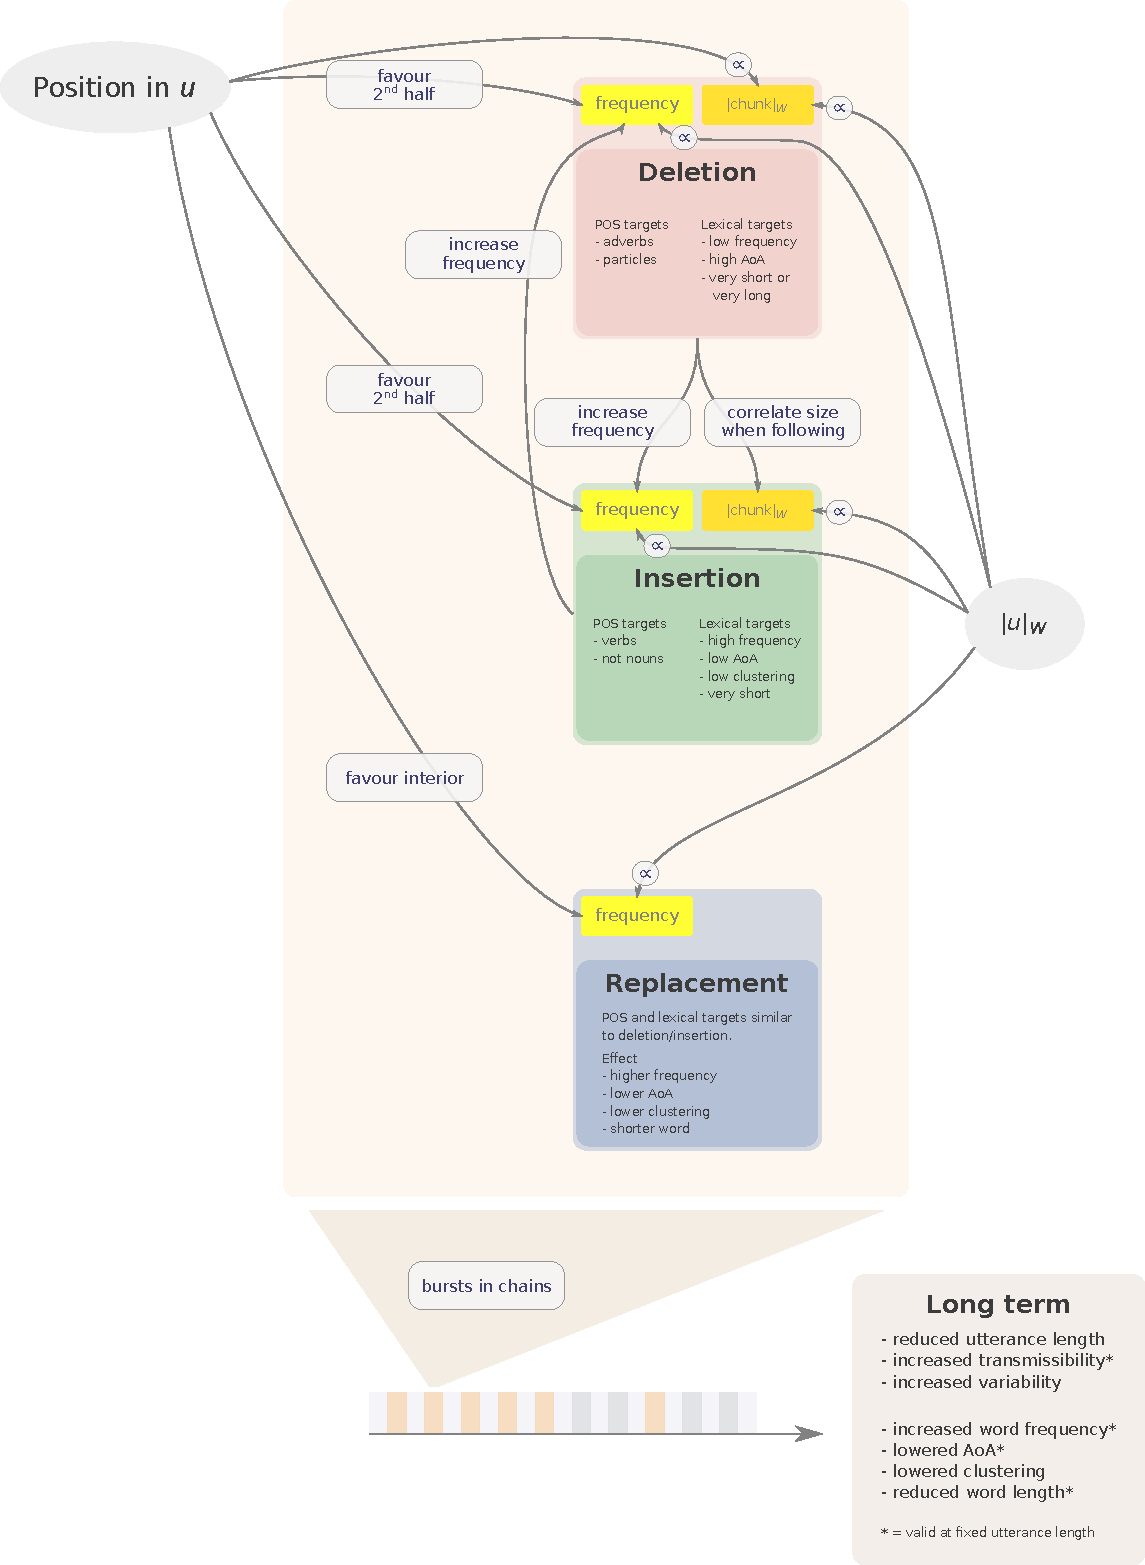
\includegraphics[width=\linewidth]{images/manual/gistr-summary.pdf}
  \caption[Summary of results]{
  \textbf{Summary of results.}
  The upper part of the figure pictures the dependencies observed in the detail of transformations.
  Transformations can be made of deletions, insertions and replacements.
  Deletions and insertions may appear in chunks, but replacements do not.
  Two main factors were shown to influence the likelihood of an operation in a given area of an utterance:
  the position of the words considered for transformation in the utterance, and the overall length of the utterance transformed.
  Arrows thus connect each factor to the frequency and the chunk size of operations, indicating the relationship between the factor and the operation (the $\propto$ symbol indicates that frequency or chunk size is roughly proportional to the factor at the beginning of the arrow).
  Three additional arrows connect deletions and insertions directly, to render the dependencies observed between these two operations.
  A summary of the types of words targeted by each operation is provided inside the darker boxes.
  Finally, the lower part of the figure recalls that transformations appear in bursts in transmission chains, and accumulate to produce the effects summarised in the "Long term" box.
  }
  \label{fig:gistr-summary}
\end{figure}

\section{Discussion}\label{sec:gistr-discussion}

We set out to better understand the process at work in the short term
evolution of linguistic content. In an approach complementary to the
previous chapter, we decided to design a controlled experiment that
would provide the complete data needed to model the process. We
developed an online platform for the purpose, and after adjusting task
difficulty and source complexity we were able to gather relatively large
data sets of linguistic transmission chains with low levels of spam.
Then, by combining standard NLP methods with our extension of a
biological sequence alignment algorithm, we decomposed the utterance
transformation process into small, analysable operations that subjects
use in their reformulations.

A few important points are worth noting to qualify the results we just
presented. First, several choices in the alignment procedure we followed
are sub-optimal, and were made in the interest of concrete progress. The
Needleman-Wunsch algorithm we used does not allow the detection of chunk
replacements. For instance, abbreviations or short paraphrases, which
\textcite{lauf_analyzing_2013} identify as non-negligible in their data
set (e.g. \enquote{has no idea} \(\rightarrow\) \enquote{doesn't know}),
are not captured by our approach. Extending the algorithm to allow this
is technically possible, but involves a substantial amount of additional
work, and we opted to leave such extensions for further research. The
algorithm is also blind to syntactic boundaries such as punctuation,
which insertions and deletions are likely to respect at least part of
the time. Manual inspection of the alignments showed a few cases where a
deletion would affect two contiguous parts of an utterance separated by
a comma, for which distinguishing the parts could help in improving the
final alignment. Finally, deep alignments are only explored on the basis
of optimal shallow alignments, which are not guaranteed to be the best
starting point: it is possible that the search will find a locally
optimal alignment, when a better solution could have been found by
starting from other (non-optimal) shallow alignments. Many other
improvements could be made in the future, for instance matching
insertion-deletion blocks from exchanges at different depths to overcome
local optima, or starting with local instead of global shallow
alignments. The manual evaluation of alignments indicated that the
current approach was good enough however, and that these optimisations
could indeed be left for further research without jeopardising our
model.

Concerning the design of the task, we note that the incentive provided
for subjects to perform well also leaves room for improvement (a point
related to the spam levels). Subjects had a monetary incentive with
bonuses for outstanding performance, but they did not experience the
bonus until after the experiment was completed. More generally, the
setup puts participants in the position of a subject and not of a user:
setting aside what the interface encourages, there is no intrinsic
incentive for people to put extra effort into the task. As
\textcite{gauld_experiments_1967} phrased it already long ago:
\enquote{Errors could, it seemed, be avoided, if the subject was so
inclined.} However, analysing the transformation rates of individual
subjects showed nothing to that effect: although some subjects average
better than others, it seems that no individual subject is uniformly
good or bad at the task. Initial explorations of the word span of
subjects (in Experiment 1) also showed little to no correlation to
subject performance. The best solution to this problem would be to
create an intrinsic motivation for the participants by aligning their
interests with performance. \textcite{claidiere_argumentation_2017}
implement this kind of incentive, by asking participants to defend and
convince others of a choice they have previously made. In our case, such
an incentive could guarantee subjects' involvement but would not suffice
to improve the quality of the written productions, as people will very
easily understand badly edited text in the course of a live interaction
(this would make the computational analysis even harder).

Finally, our setup entirely obviates the question of the context in
which utterances are processed and reproduced. This was a deliberate
choice, as we decided to use the simplest transmission chain task
possible and reserve the introduction of more complexity (such as
context effects) for later research. As a consequence however, we have
no control over the situation in which subjects read an utterance, nor
did we add contextual paragraphs or preceding utterances to examine
framing or priming effects on the interpretations and transformations
made by subjects. Preceding text is very likely to have effects on the
transformations, as these are reliably observed in the study of
intrusions in recall of word lists \autocite{zaromb_temporal_2006}.
Manual exploration of the data also showed (rare) cases of words from
one utterance bleeding into later transformations: in one case, a
subject reintroduced a word that they had read in an utterance three
trials earlier. This phenomenon is difficult to control beyond the
randomisation we applied, and we note that the cases we observed were
extremely rare.

In spite of these caveats, we showed that transformations can be
usefully analysed as made of bursty deletions and insertions, speckled
with word replacements (and exchanges, which we left aside in the
analysis). Deletions are by far the most frequent operation, and they
act as a gate for insertions; in turn, the size of insertions tends to
correlate to the size of deletions that they closely follow. We further
observed that all operations are less probable at the beginning of an
utterance, as well as in shorter utterances, and that deletions tend to
grow in chunk size as well as in chunk numbers towards the end of an
utterance. Finally, we observed that transformations are also bursty at
the level of the branch, suggesting that the process follows a
punctuated equilibria pattern: when a subject makes a transformation on
a previously stable utterance, the next subjects in the chain might add
transformations until the changes are regularised into a newly stable
utterance.

Overall, we suggest that adopting this descriptive model provides a
clearer picture of the process at work in the evolution of linguistic
content than has been previously achieved. The model creates an
intermediary scale between the detailed level of lexical word features
and the high level of contrasts in aggregated evolution, thus rendering
the process more intelligible. In particular, we believe that
visualisations such as the lineage plots we presented are extremely
helpful in identifying the underlying mechanisms that can be then
connected to known effects in linguistics. In the context of Cultural
Attraction Theory, this type of approach could prove useful to construct
more parsimonious models of the evolution of representations. In
particular, it brings detail to the linguistic instantiation of the
wear-and-tear and flop problems introduced by \textcite{morin_how_2016}:
the first could correspond to the way utterances are gradually
transformed by replacements, exchanges, and insertions making up for
deletions; the second could correspond to downright mass deletions in a
transformation.

Transposing the analysis from the previous chapter to the current data
set also confirmed the trends in lexical features observed in blogspace:
less frequent, longer words that are learned late and have higher
clustering coefficient are on average replaced by higher-frequency,
shorter words, learned earlier and with lower clustering coefficient. As
we discussed in the previous chapter, these words are overall easier to
produce in standard naming or word recall tasks. Examining the evolution
of these features along the branches also showed that the process
significantly transforms utterances to use easier words on average:
transformations can thus be seen as creating a gradual drift of
utterances at the low-level of lexical features due to a cognitive bias
in favour of certain word types.

While one could consider this phenomenon as relevant to Cultural
Attraction Theory, it remains extremely low-level and does not indicate
any consistent drift or attraction in the semantics of the utterances
(nor does it invalidate it). Manual inspection of the data also gave no
sign of an attraction phenomenon at the semantic level. Two points might
be noted nonetheless. First, the details of transformations seem to
follow the patterns identified by \textcite{lauf_analyzing_2013} in news
stories: complements, adverbs, modals, and more generally any details
not essential to the main meaning seem often deleted or replaced.
Second, examining episodes of bursty changes also suggested that there
is a chaotic aspect to chains: relatively minor changes in the middle of
a transformation sometimes lead to a comparatively larger change in
meaning down the branch, as an ambiguity is created and resolved
differently than previously. In Experiment 3 for instance, a subject
presented with the following utterance,

\begin{nquote} % <!-- #545 -->
  "A dozen hawkers who had been announcing the news of a non existent bomber in Kings Cross have been arrested."
\end{nquote}

introduced several changes including a typographical error that replaced
the word \enquote{news} with \enquote{new}; he or she produced the
following utterance:

\begin{nquote} % <!-- #907 -->
  "A dozen hawkers announcing non existent \textbf{new} about a bomber at Kings Cross have been arrested"
\end{nquote}

The \enquote{news} \(\rightarrow\) \enquote{new} change, while
superficially minor compared to the rest of the transformation, is quite
important once we remove the context provided by the previous utterance.
Indeed, it later went through a long regularisation such that the final
utterance of the branch read:

\begin{nquote} % <!-- #1847 -->
  "A dozen hawkers, at New Kings Cross have been arrested."
\end{nquote}

Examining the transformations in the branch suggested that the small
typographical error rendered its surroundings (\enquote{non existent
\ldots{} about a bomber}) confusing and irrelevant, such that
\enquote{new} was finally integrated as part of the \enquote{Kings
Cross} proper noun instead. This behaviour is not frequent, as many
times typographical errors are corrected by subsequent transformations,
but it appears to be possible whenever an ambiguity is created or
enhanced (not only through typographical errors).

Other intriguing semantic effects were observed. In one case for
instance, small changes that accumulated in different parts of an
utterance ended up combining into a larger semantic change, because the
relationship between parts of the utterance had eventually changed. More
broadly, tackling the question of semantic attraction (or more simply
semantic transformations) could require the definition of semantic
levels at which the transformations should be examined. As the chaotic
behaviour described above illustrates, changes at the semantic level can
be created by any ambiguity that is picked up by subjects. This can
range from a typographical error, to a change in punctuation, or a minor
change of vocabulary which seems ambiguous to one subject but not to
another. The question is thus shifted from the structure of utterances
themselves to what subjects attend to, in an utterance, for a given task
or in a given interaction situation. In other words, analysing the
semantic changes of utterances goes hand in hand with a determination of
what aspects of an utterance are relevant for a given task or
interaction, that is, it requires an approach to utterance pragmatics.

Without delving into utterance pragmatics, a more palatable development
of this approach would be to focus on a smaller number of root
utterances with less branches in each tree, and explore evolution of
content at the very long term. While such an approach would be more
dependent on the initial utterances, it would allow us to explore
higher-level evolutionary dynamics along the chain (e.g.~recurring sets
of changes). Testing for the existence of attractors, in particular,
might require such long-lived chains, as the number of iterations is an
important factor to consider. A second approach, which could be combined
with long-lived chains, would be to ask about the role of simple
semantics and syntax in the transformations: beyond lexical features and
word categorisations, one could attempt to quantify and thus
characterise the change in meaning at each transformation and overall
through the chains, possibly through deeper integration with existing
NLP methods. Semantic parsing methods, in particular, can provide a
first useful model of the semantics encoded in a sentence. Depending on
the way such information is represented, an alignment technique similar
to the one developed here could be used to study the changes in semantic
parses along a chain, thus opening the study of the regularities in
semantic transformations. Conversely, the extent to which word meanings
(or word relationships with the rest of the utterance) participate in
the transformation process could be explored. Better integrating these
results with what is known of the way utterances are cognitively
processed and produced could also be fruitful: known mechanisms in
sentence parsing and processing could explain the patterns observed by
our model, and integrating with current knowledge of sentence production
could make it possible to develop generative models of the
transformation process. Finally, many questions from the last chapter
also remain pending. In particular, if context is an important factor in
the transformations observed, we wonder about the role of feedback
effects and path dependence in the evolution of content online: how much
are transformations determined by the distribution of utterances that
readers are exposed to, in what way, and how does this influence feed
back into the distribution itself? An important role of feedback in the
transformations would be grounds for a strong path dependence in the
evolution of linguistic content, maybe even at lower cognitive levels.

Answering these more approachable questions would already provide a much
more complete view of the dynamics at work in the short-term evolution
of linguistic content. As noted above however, it is likely that further
progress in this area will require considering the role of pragmatics in
utterance transformations, for instance by exploring more ecological
interaction situations than the simple read-and-rewrite task we used.


% Some final thanks and stuff
\subsection*{Acknowledgements}
\rk{todo}

\subsection*{Software colophon}
\rk{todo}


\printbibliography

\appendix
\section{Varia}

\begin{algorithm}
\caption{An implementation of the deep alignment extension for detecting exchanges in NW alignments.
Note that this implementation is less efficient but presentationally clearer than the implementation we made.
}
\label{alg:deep-alignment}
\begin{algorithmic}
\Function{shallowalign}{$u$, $u'$}
  \State (Implemented by Biopython)
  \State \Return List of optimal shallow alignments of $u$ and $u'$
\EndFunction \\

\Function{mappings}{$a_{shallow}$}
  \State $\mathcal{D}\gets \{d | d\text{ deletion block in }a_{shallow}\}$
  \State $\mathcal{I}\gets \{i | i\text{ deletion block in }a_{shallow}\}$
  \State \Return $\mathcal{D}^{P(\mathcal{I})}$ \Comment{$P(\Omega)$ is the power set of $\Omega$}
\EndFunction \\

\Function{scoremapping}{$a_{shallow}$, $D_M$}
  \State $s\gets 0$
  \For{$((u_{e,-,} u_{e,+}), D_e)$ in $D_M$}
    \State $s\gets s + \theta_{exchange}$
    \State $s\gets s - \Call{score}{\text{deletion of }u_{e,-}} - \Call{score}{\text{insertion of }u_{e,+}}$
    \State $s\gets s + \max\{\chi_{deep}(a_{deep}) | a_{deep} \in D_e\}$
  \EndFor
  \State \Return $s$
\EndFunction \\

\Function{deepalign}{$u$, $u'$}
  \State $D\gets []$ \Comment{$D$ is the list of deep alignments trees we have explored}
  \For{$a_{shallow}$ shallow alignment in \Call{shallowalign}{$u$, $u'$}}
    \If{$a_{shallow}$ has no gaps or has only gaps}
      \State $D\gets (a_{shallow}, [], \chi_{shallow}(a_{shallow}))$
    \Else
      \For{$M$ mapping in \Call{mappings}{$a_{shallow}$}}
        \State $D_M\gets []$
        \For{$(u_{e,-}, u_{e,+})$ exchange in $M$}
          \State $D_M\gets D_M + ((u_{e,-}, u_{e,+}), \Call{deepalign}{u_{e,-}, u_{e,+}})$
        \EndFor
        \State $D\gets D + (a_{shallow}, D_M, \chi_{shallow}(a_{shallow}) + \Call{scoremapping}{a_{shallow}, D_M})$
      \EndFor
    \EndIf
  \EndFor
  \State \Return Recursively pruned version of $D$ with only maximally scoring deep alignments
\EndFunction
\end{algorithmic}
\end{algorithm}

\end{document}
